\documentclass[class=smolathesis,crop=false]{standalone}

\begin{document}

\chapter{Process Compositions as Port Graphs}
\label{ch:port_graphs}

In Chapter~\ref{ch:proc} we introduced process compositions that formally described how a process is formed from smaller ones by means of simple operations.
The core information that we can extract from process compositions is how individual actions in the process connect through the resources they produce and consume.
In Section~\ref{sec:proc/diag} we introduced process diagrams, visualising process compositions from this point of view.
They represent actions as boxes, which are connected by wires to represent resource dependencies.
While this visualisation is useful for concisely communicating the composition, it is done outside of the proof assistant.
As a result, it is not fully rigorous: we make no formal connection between the composition tree and the diagram beyond the Haskell function drawing it.
More specifically, we cannot formally verify any claims about the visualisation or use it in proofs.

In this chapter we make more rigorous the connection between composition trees, which can be seen as the ``algebraic'' representation, and process diagrams, which can be considered to be the ``graphical'' representation.
For this, we mechanise in Isabelle/HOL \emph{port graphs}, the notion that underpins our process diagrams.
We then define a mapping from process compositions into port graphs and formally verify a number of its properties.
See Figure~\ref{fig:cargo_port_graph} for an illustrative port graph constructed by our framework to represent a manufacturing process composition.

\begin{figure}[htbp]
  \centering
  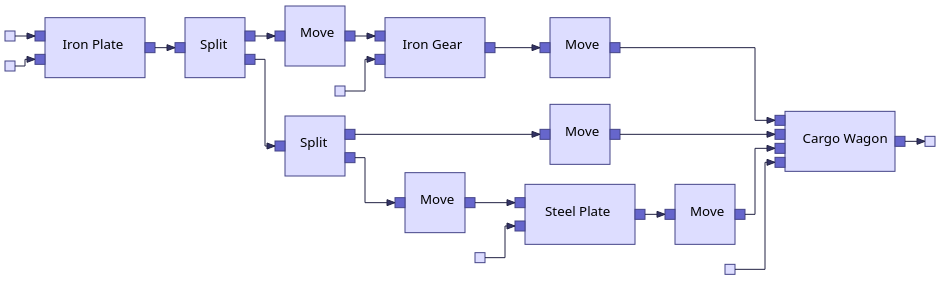
\includegraphics[width=\textwidth]{img/cargo_port_graph.png}
  \caption{
    Visualisation of a port graph constructed by our framework to represent a composition from a manufacturing domain (see Section~\ref{sec:cases/factorio} for a discussion of that domain).
    The composition has 11 primitive actions, represented here by nodes.
    Composition operations and resource actions yield the connections between ports of those nodes, representing resources.
  }
  \label{fig:cargo_port_graph}
\end{figure}

Our verification culminates in a graphical characterisation of composition linearity and its proof for every valid composition.
It serves as a counterpart to Chapter~\ref{ch:linearity}, where linearity is demonstrated by appealing to linear logic.
This characterisation of linearity specifies more directly which connections between actions are allowed.

At present, our approach is limited to sequential and parallel process compositions, because we find the base form of port graphs insufficient for expressing non-deterministic and higher-order features.
As a result, we do not provide a port graph mapping for optional composition, process representation or their associated resource actions (such as \isa{InjectL} and \isa{Apply}).
The most direct strand of future work, outlined in Section~\ref{sec:port_graphs/conc}, aims to extend port graphs and their mechanisation to cover such features and allow for a fully formal graphical representation of \emph{all} process compositions.

The remainder of this chapter proceeds as follows.
In Section~\ref{sec:port_graphs/rel} we highlight some related work on port graphs and then in Section~\ref{sec:port_graphs/pg} we introduce the notion of port graphs with a focus on the aspects relevant to our mechanisation.
In Section~\ref{sec:port_graphs/mech} we describe our mechanisation of port graphs in general, which forms a self-contained theory that can be reused for other applications.
Then in Section~\ref{sec:port_graphs/process} we give our mapping of process compositions to a specific kind of port graphs and discuss some of its basic properties.
In Section~\ref{sec:port_graphs/interchange} we use port graphs to prove when sequential and parallel process composition operations distribute over each other.
In Section~\ref{sec:port_graphs/linearity} we use port graphs to characterise process linearity in terms of allowed connections between actions, and prove it to hold for valid process compositions.
In Section~\ref{sec:port_graphs/trans} we define a transition system for port graphs, showing that equivalent port graphs have equivalent transitions.
This gives a behavioural dimension to equivalences between port graphs that we prove in prior sections.
Finally, in Section~\ref{sec:port_graphs/conc} we give concluding remarks and outline future work.

\section{Related Work}
\label{sec:port_graphs/rel}

Port graphs and port graph rewriting systems have been used to model various complex systems.
For instance, Andrei et al.~\cite{andrei_et_al-2011} use them to model biochemical processes and Vallet et al.~\cite{vallet_et_al-2015} use them to model social networks.
In comparison to ordinary graphs, the advantage of port graphs is that they allow us to model the specific points where edges connect to nodes.
This is useful to represent, for instance, protein sites in biochemistry or communication ports in computer networks.
In our case, they are crucial to representing specific input and output resources of individual actions.

Port graphs are also connected to graphical representations arising in applications of category theory.
In their book on applied category theory, Fong and Spivak~\cite{fong_spivak-2019} use port graphs in their formalisation of signal flow graphs, a graphical language used for instance in signal processing.
As shown for instance by Bonchi et al.~\cite{bonchi_et_al-2015}, signal flow graphs can be viewed as string diagrams, which are widely used in the study of monoidal categories~\cite{maclane-1998}.
Through monoidal categories, string diagrams connect to a wide range of graphical representations in applied category theory, such as the ZX calculus in the study of quantum circuits~\cite{coecke_duncan-2008,kissinger_zamdzhiev-2015}.
As such, there is evidence for the fruitful use of port graphs to formalise graphical representations.

Note that, in the literature, port graphs are often formalised with a set of nodes, a set of ports and a function from ports to nodes expressing to which node each port is attached.
In our mechanisation we diverge from this representation and instead formalise the ports attached to each node as part of that node.
This means that, in mechanising operations on port graphs, we are modifying collections instead of updating functions.
We find this approach to be easier to verify.
Nevertheless, we can recover the attachment function from our formalisation and, as such, we do not lose anything by using our approach.

Another use of port graphs is the Incredible Proof Machine~\cite{breitner_2016}, a tool for visual construction of proofs.
It uses port graphs to represent proofs, with nodes representing inference rules and ports their premises and conclusions.
Notably, the meta theory of this tool is verified in Isabelle/HOL~\cite{Incredible_Proof_Machine-AFP}.
As far as we are aware, this is the only published mechanisation of port graphs.
However, it is specific to their use as part of the tool being verified.
For instance, they do not support open ports, which we find vital to defining operations connecting multiple port graphs (see Section~\ref{sec:port_graphs/mech/seq}).
Instead of adapting this mechanisation, we choose to develop our own.

\section{Port Graphs}
\label{sec:port_graphs/pg}

Port graphs~\cite{andrei_2008} refine the notion of directed graphs.
Recall that the latter consist of a collection of nodes and a collection of edges going from one node to another.
(Undirected graphs simply discard the distinction between edge origin and destination.)

\begin{figure}[htbp]
  \centering
  \includesvg[scale=0.5]{img/pg_intro_0}
  \caption{Example directed graph with three nodes and three edges}
  \label{fig:pg_intro_0}
\end{figure}

As suggested by their name, port graphs modify directed graphs with \emph{ports} to mediate the connection between nodes and edges.
They are still formed by collections of nodes and edges, but every node has a collection of ports attached to it and edges go between ports instead of the nodes themselves.
Note that this does not require all ports to have an adjacent edge.
The ports allow us to express where and how nodes are connected, instead of simply saying that they are connected or not.

In practice, these ports have been used to express sites on proteins when representing biological processes~\cite{andrei_et_al-2011}, or input and output signals in signal flow graphs~\cite{fong_spivak-2019}.

\begin{figure}[htbp]
  \centering
  \includesvg[scale=0.5]{img/pg_intro_1}
  \caption{Example port graph with three nodes, three edges and eight ports, two of which are left unconnected}
  \label{fig:pg_intro_1}
\end{figure}

Note that it is possible to turn any port graph into a directed graph, essentially forgetting the connection details that the ports express.
We can do this by taking the same range of nodes as the port graph and then, for every edge of the port graph we ensure there is an edge in the directed graph that goes from the originating port's node to the destination port's node.
If the port graph edges express dependencies, as they do for our process port graphs, then the directed graph constructed in this way can be used to check for dependency loops.
We make use of this when discussing a transition system for port graphs in Section~\ref{sec:port_graphs/trans} to show when it terminates.
This graph is sometimes called the \emph{internal flow graph}~\cite{fong_spivak-2019}.

\emph{Labelled} port graphs~\cite{fernandez_et_al-2019} extend this idea further by labelling each node, port and edge with arbitrary data.
This is of great practical use when the port graph is used to represent additional information.
For instance, a representation of a distributed system may label nodes with IP addresses and ports with port numbers.

\begin{figure}[htbp]
  \centering
  \includesvg[scale=0.5,pretex=\relscale{0.8}\tt]{img/pg_intro_lab}
  \caption{Example port graph with simple text labels on nodes and ports}
  \label{fig:pg_intro_lab}
\end{figure}

In our case we use node and port labels for multiple purposes.
We name nodes based on the corresponding primitive action's position in the composition to uniquely identify them and we annotate them with its label and metadata.
We label ports with a combination of side (e.g.\ input and output for processes) and index to uniquely identify them in their collections and we annotate them with the resources they carry.

\emph{Open} port graphs address connecting port graphs to form larger ones.
They add a number of ports not attached to any node, which we may call \emph{open}, that are available for connection from some outside environment.
Then two port graphs may be combined by describing how their open ports are to be connected to form new edges.
\cbar{Note that having open ports not attached to any node allows us to have meaningful port graphs with no nodes.
These are useful when combining port graphs, for instance to reorder how existing edges connect to open ports or to disconnect some of them.}

\begin{figure}[htbp]
  \centering
  \includesvg[scale=0.5,pretex=\relscale{0.8}\tt]{img/pg_intro_open}
  \caption{Example labelled port graph with port \texttt{c2} connected to the open port \texttt{p}}
  \label{fig:pg_intro_open}
\end{figure}

This variant is useful when reasoning about port graphs in category theory, where it is vital to have a notion of interface (which here would be the collection of open ports) and composition~\cite{fong_spivak-2019}.

In our case, we use open ports for the input and output resources of the process being represented.
Sequential process composition then uses those open ports to form the relevant new connections.

\emph{Hierarchical} port graphs~\cite{ene_et_al-2018} allow for nodes to contain whole other port graphs within them.
As the name suggests, these are useful for going beyond connection and representing hierarchical structure as well.
This allows them to represent multi-layer systems as well as representing multiple layers of abstraction.

At present, we do not mechanise hierarchical port graphs or make use of them to represent process compositions.
However, their existence suggests a future extension to our mechanisation of port graphs that may improve the range of features they can express.
See Section~\ref{sec:port_graphs/conc} for our discussion of future work.

In the next section we describe our mechanisation of open port graphs with port and node labels.
We then use this theory in succeeding sections to graphically represent process compositions and verify properties about connections between individual actions.

\section{Mechanisation of Port Graphs}
\label{sec:port_graphs/mech}

We mechanise port graphs in two parts: their data and the constraints on that data.
We then define operations on the data and verify that they preserve those constraints (among other properties).

The data itself we represent using a datatype, which gathers the nodes, edges and open ports.
To make implementing operations on port graphs simpler, we use lists for all three collections to represent finite sets.

The constraints on the data we represent as locales, which are Isabelle's construct for collecting together assumptions and the facts stemming from them.
This means that if the data satisfies the locale assumptions, then the facts of the locale are true of the data.

The operations we define are ultimately in service of graphically representing process compositions.
However, we keep this part of the theory more general to make it reusable in other contexts.

\subsection{Ports}
\label{sec:port_graphs/mech/ports}

Before we state exactly how the data is represented, recall from Section~\ref{sec:proc/diag/paths} our definition of (qualified) ports (reproduced in Definition~\ref{isa:port+qualified}).
\cbar{We will now be using their general definitions to mechanise port graphs that allow for any port sides, labels and qualifying atoms.
In Section~\ref{sec:port_graphs/process/prelim} we then specialise these type variables in the same way we did for process diagrams in Section~\ref{sec:proc/diag/paths} to yield process port graphs.
That is, we will use input and output as port sides, resources as port labels and composition tree paths as atoms qualifying the ports.}

\begin{isadef}[Datatypes of ports and qualified ports]{isa:port+qualified}
  \isacomm{datatype}\isamarkupfalse%
\ {\isacharparenleft}\isatv{s}{\isacharcomma}\ \isatv{a}{\isacharparenright}\ port\ {\isacharequal}\ Port\ {\isacharparenleft}\isafv{side}{\isacharcolon}\ \isatv{s}{\isacharparenright}\ {\isacharparenleft}\isafv{index}{\isacharcolon}\ nat{\isacharparenright}\ {\isacharparenleft}\isafv{label}{\isacharcolon}\ \isatv{a}{\isacharparenright}

\item
  \isacomm{datatype}\isamarkupfalse%
\ {\isacharparenleft}\isatv{s}{\isacharcomma}\ \isatv{a}{\isacharcomma}\ \isatv{p}{\isacharparenright}\ qualified{\isacharunderscore}port\ {\isacharequal}\ QPort\ {\isacharparenleft}\isafv{port}{\isacharcolon}\ {\isachardoublequoteopen}{\isacharparenleft}\isatv{s}{\isacharcomma}\ \isatv{a}{\isacharparenright}\ port{\isachardoublequoteclose}{\isacharparenright}\ {\isacharparenleft}\isafv{name}{\isacharcolon}\ {\isachardoublequoteopen}\isatv{p}\ list{\isachardoublequoteclose}{\isacharparenright}

\end{isadef}

Note that names are sequences of atoms rather than simply an arbitrary type.
This allows us to further qualify an already qualified port with an additional atom.
When done to two collections of ports with two distinct atoms, this allows us to easily make those two collections disjoint.
For qualified ports, this operation is defined as follows:
\begin{isadef}[Further qualifying a qualified port]{isa:qualifyQPort}
  \isacomm{primrec}\isamarkupfalse%
\ qualifyQPort\ {\isacharcolon}{\isacharcolon}\ {\isachardoublequoteopen}\isatv{p}\ {\isasymRightarrow}\ {\isacharparenleft}\isatv{s}{\isacharcomma}\ \isatv{a}{\isacharcomma}\ \isatv{p}{\isacharparenright}\ qualified{\isacharunderscore}port\ {\isasymRightarrow}\ {\isacharparenleft}\isatv{s}{\isacharcomma}\ \isatv{a}{\isacharcomma}\ \isatv{p}{\isacharparenright}\ qualified{\isacharunderscore}port{\isachardoublequoteclose}\isanewline
\ \ \isaOcomm{where}\ {\isachardoublequoteopen}\isafv{qualifyQPort}\ \isabv{x}\ {\isacharparenleft}QPort\ \isabv{port\ path}{\isacharparenright}\ {\isacharequal}\ QPort\ \isabv{port}\ {\isacharparenleft}\isabv{x}\ {\isacharhash}\ \isabv{path}{\isacharparenright}{\isachardoublequoteclose}

\end{isadef}

\subsection{Nodes, Edges and Places}
\label{sec:port_graphs/mech/parts}

Nodes, edges and places are the different parts of port graphs.
While the first two represent exactly those basic graph components, places represent the union of both ports attached to nodes (which we call \emph{ground} ports) and open ports, which are not attached to a node.
In other words, places are what edges can connect.

Nodes are formed from a name (again a sequence of atoms drawn from type \isa{\isatv{p}}), a label drawn from type \isa{\isatv{l}} and the ports attached to the node (themselves drawing sides from type \isa{\isatv{s}} and labels from type \isa{\isatv{a}}).
Mechanised in Isabele/HOL:
\begin{isadef}[Datatype of nodes]{isa:node}
  \isacomm{datatype}\isamarkupfalse%
\ {\isacharparenleft}\isatv{s}{\isacharcomma}\ \isatv{a}{\isacharcomma}\ \isatv{p}{\isacharcomma}\ \isatv{l}{\isacharparenright}\ node\ {\isacharequal}\isanewline
\ \ Node\ {\isacharparenleft}\isafv{node{\isacharunderscore}name}{\isacharcolon}\ {\isachardoublequoteopen}\isatv{p}\ list{\isachardoublequoteclose}{\isacharparenright}\ {\isacharparenleft}\isafv{node{\isacharunderscore}label}{\isacharcolon}\ \isatv{l}{\isacharparenright}\ {\isacharparenleft}\isafv{node{\isacharunderscore}ports}{\isacharcolon}\ {\isachardoublequoteopen}{\isacharparenleft}\isatv{s}{\isacharcomma}\ \isatv{a}{\isacharparenright}\ port\ list{\isachardoublequoteclose}{\isacharparenright}

\end{isadef}
Note that in Section~\ref{sec:port_graphs/process/prelim}, when specifying port graphs for process compositions, we instantiate the node labels to carry the labels and metadata of primitive actions.

Places can be either ground ports, qualified by a node name, or open ports.
We mechanise them in Isabelle/HOL as follows (with type variables \isatv{s}, \isatv{a} and \isatv{p} again just as with qualified ports):
\begin{isadef}[Datatype of places]{isa:place}
  \isacomm{datatype}\isamarkupfalse%
\ {\isacharparenleft}\isatv{s}{\isacharcomma}\ \isatv{a}{\isacharcomma}\ \isatv{p}{\isacharparenright}\ place\ {\isacharequal}\isanewline
\ \ \ \ place{\isacharunderscore}ground{\isacharcolon}\ GroundPort\ \isapars{{\isachardoublequoteopen}{\isacharparenleft}\isatv{s}{\isacharcomma}\ \isatv{a}{\isacharcomma}\ \isatv{p}{\isacharparenright}\ qualified{\isacharunderscore}port{\isachardoublequoteclose}}\isanewline
\ \ {\isacharbar}\ place{\isacharunderscore}open{\isacharcolon}\ OpenPort\ \isapars{{\isachardoublequoteopen}{\isacharparenleft}\isatv{s}{\isacharcomma}\ \isatv{a}{\isacharparenright}\ port{\isachardoublequoteclose}}

\end{isadef}
The automatically generated predicates \isa{place{\isacharunderscore}ground} and \isa{place{\isacharunderscore}open} allow us to easily distinguish the two kinds of places, which is a frequent point in proofs.

With both nodes and places defined, we can for instance define how all the ground places induced by a node can be collected:
\begin{isadef}[Collecting ground places of a node]{isa:nodePlaces}
  \isacomm{fun}\isamarkupfalse%
\ nodePlaces\ {\isacharcolon}{\isacharcolon}\ {\isachardoublequoteopen}{\isacharparenleft}\isatv{s}{\isacharcomma}\ \isatv{a}{\isacharcomma}\ \isatv{p}{\isacharcomma}\ \isatv{l}{\isacharparenright}\ node\ {\isasymRightarrow}\ {\isacharparenleft}\isatv{s}{\isacharcomma}\ \isatv{a}{\isacharcomma}\ \isatv{p}{\isacharparenright}\ place\ list{\isachardoublequoteclose}\isanewline
\ \ \isaOcomm{where}\ {\isachardoublequoteopen}\isafv{nodePlaces}\ \isabv{n}\ {\isacharequal}\isanewline
\ \ \ \ map\ {\isacharparenleft}{\isasymlambda}\isabv{p}{\isachardot}\ GroundPort\ {\isacharparenleft}QPort\ \isabv{p}\ {\isacharparenleft}node{\isacharunderscore}name\ \isabv{n}{\isacharparenright}{\isacharparenright}{\isacharparenright}\ {\isacharparenleft}node{\isacharunderscore}ports\ \isabv{n}{\isacharparenright}{\isachardoublequoteclose}%

\end{isadef}

Edges are made up of two places, the origin and destination, meaning they are simple and directed edges.
Mechanised in Isabelle/HOL (with type variables \isatv{s}, \isatv{a} and \isatv{p} again just as with qualified ports):
\begin{isadef}[Datatype of edges]{isa:edge}
  \isacomm{datatype}\isamarkupfalse%
\ {\isacharparenleft}\isatv{s}{\isacharcomma}\ \isatv{a}{\isacharcomma}\ \isatv{p}{\isacharparenright}\ edge\ {\isacharequal}\isanewline
\ \ Edge\ {\isacharparenleft}\isafv{edge{\isacharunderscore}from}{\isacharcolon}\ {\isachardoublequoteopen}{\isacharparenleft}\isatv{s}{\isacharcomma}\ \isatv{a}{\isacharcomma}\ \isatv{p}{\isacharparenright}\ place{\isachardoublequoteclose}{\isacharparenright}\ {\isacharparenleft}\isafv{edge{\isacharunderscore}to}{\isacharcolon}\ {\isachardoublequoteopen}{\isacharparenleft}\isatv{s}{\isacharcomma}\ \isatv{a}{\isacharcomma}\ \isatv{p}{\isacharparenright}\ place{\isachardoublequoteclose}{\isacharparenright}

\end{isadef}

We now illustrate these constructs before using them in port graphs.
\cbstart
Consider the \isa{add{\isacharunderscore}to{\isacharunderscore}credit} action from Definition~\ref{isa:add_to_credit}, say with existing credit of zero and adding ten in cash.
This action has two input atoms (\isa{Machine\ 0} and \isa{Cash\ 10}) and one output atom (\isa{Machine\ 10}).
Let this action be found as the first child under two sequential compositions, such as in the example in Section~\ref{sec:proc/type/res}.
While our full process port graph construction uses more complex labels (described in Section~\ref{sec:port_graphs/process}), we could represent this action with the node:
\begin{center}
  \begin{minipage}{0.75\textwidth}
    \begin{isabelle}
      Node\ \isalist{SeqL,\ SeqL}\isanewline
      \isaindent{Node\ }\isaString{Add\ to\ credit}\isanewline
      \isaindent{Node\ }\isalist{Port\ In\ \isadigit{0}\ \isapars{Res\ \isapars{Machine\ 0}},\ Port\ In\ \isadigit{1}\ \isapars{Res\ \isapars{Cash\ 10}},\isanewline
      \isaindent{Node\ {\isacharbrackleft}}Port\ Out\ \isadigit{0}\ \isapars{Res\ \isapars{Machine\ 10}}}
    \end{isabelle}
  \end{minipage}
\end{center}
and one of its places would then be:
\begin{isabelle}
\centering
  GroundPort\ \isapars{QPort\ \isapars{Port\ In\ \isadigit{0}\ \isapars{Res\ \isapars{Machine\ 0}}}\ \isalist{SeqL,\ SeqL}}
\end{isabelle}
Then, if this node was within a larger port graph that has the following open input port:
\begin{isabelle}
\centering
  Port\ In\ \isadigit{3}\ \isapars{Res\ \isapars{Machine\ 0}}
\end{isabelle}
we could connect this open port to the node's input with the following edge:
\begin{isabelle}
\centering
  Edge\ \widthtoR{\isapars{OpenPort\ \isapars{Port\ In\ \isadigit{3}\ \isapars{Res\ \isapars{Machine\ 0}}}}}{\isapars{GroundPort\ \isapars{QPort\ \isapars{Port\ In\ \isadigit{0}\ \isapars{Res\ \isapars{Machine\ 0}}}\ \isalist{SeqL,\ SeqL}}}}\isanewline
  \isaindent{Edge\ }\isapars{GroundPort\ \isapars{QPort\ \isapars{Port\ In\ \isadigit{0}\ \isapars{Res\ \isapars{Machine\ 0}}}\ \isalist{SeqL,\ SeqL}}}
\end{isabelle}
\cbend

\subsection{Port Graph Data}
\label{sec:port_graphs/mech/data}

With all the constituent parts defined, we can now mechanise the port graph data itself, with sides drawn from type \isa{\isatv{s}}, port labels drawn from type \isa{\isatv{a}}, name atoms drawn from type \isa{\isatv{p}} and node labels drawn from type \isa{\isatv{l}}:
\begin{isadef}[Datatype of port graphs]{isa:type-port_graph}
  \isacomm{datatype}\isamarkupfalse%
\ {\isacharparenleft}\isatv{s}{\isacharcomma}\ \isatv{a}{\isacharcomma}\ \isatv{p}{\isacharcomma}\ \isatv{l}{\isacharparenright}\ port{\isacharunderscore}graph\ {\isacharequal}\isanewline
\ \ PGraph\ {\isacharparenleft}\isafv{pg{\isacharunderscore}nodes}{\isacharcolon}\ {\isachardoublequoteopen}{\isacharparenleft}\isatv{s}{\isacharcomma}\ \isatv{a}{\isacharcomma}\ \isatv{p}{\isacharcomma}\ \isatv{l}{\isacharparenright}\ node\ list{\isachardoublequoteclose}{\isacharparenright}\isanewline
\isaindent{\ \ PGraph\ }{\isacharparenleft}\isafv{pg{\isacharunderscore}edges}{\isacharcolon}\ {\isachardoublequoteopen}{\isacharparenleft}\isatv{s}{\isacharcomma}\ \isatv{a}{\isacharcomma}\ \isatv{p}{\isacharparenright}\ edge\ list{\isachardoublequoteclose}{\isacharparenright}\isanewline
\isaindent{\ \ PGraph\ }{\isacharparenleft}\isafv{pg{\isacharunderscore}ports}{\isacharcolon}\ {\isachardoublequoteopen}{\isacharparenleft}\isatv{s}{\isacharcomma}\ \isatv{a}{\isacharparenright}\ port\ list{\isachardoublequoteclose}{\isacharparenright}%

\end{isadef}

On this data alone we make several useful definitions: a function to qualify the whole port graph, a function to collect all places occurring in it and a relation for port graphs with no names in common.

The function \isa{qualifyPortGraph} takes a name atom and prefixes it to names of all nodes in the port graph as well as the names qualifying ground places in edges.
We define it using a series of functions with the same effect on different targets, called \isa{qualifyNode}, \isa{qualifyEdge} and \isa{qualifyPlace}, culminating in \isa{qualifyPortGraph}.
All of these either qualify their target's constituent parts or, in the case of \isa{qualifyNode}, prefix its name with the atom just as \isa{qualifyQPort} in Section~\ref{sec:port_graphs/mech/ports} does.

The function \isa{pgraphPlaces} collects all the places occurring in the port graph by combining those attached to its nodes with its open ports.
This function figures frequently in proofs about port graphs and is defined as follows:
\pagebreak
\begin{isadef}[Collecting open and ground places of a port graph]{isa:pgraphPlaces}
  \isacomm{fun}\isamarkupfalse%
\ pgraphPlaces\ {\isacharcolon}{\isacharcolon}\ {\isachardoublequoteopen}{\isacharparenleft}\isatv{s}{\isacharcomma}\ \isatv{a}{\isacharcomma}\ \isatv{p}{\isacharcomma}\ \isatv{l}{\isacharparenright}\ port{\isacharunderscore}graph\ {\isasymRightarrow}\ {\isacharparenleft}\isatv{s}{\isacharcomma}\ \isatv{a}{\isacharcomma}\ \isatv{p}{\isacharparenright}\ place\ list{\isachardoublequoteclose}\isanewline
\ \ \isaOcomm{where}\ {\isachardoublequoteopen}\isafv{pgraphPlaces}\ \isabv{x}\ {\isacharequal}\isanewline
\ \ \ \ concat\ {\isacharparenleft}map\ nodePlaces\ {\isacharparenleft}pg{\isacharunderscore}nodes\ \isabv{x}{\isacharparenright}{\isacharparenright}\ {\isacharat}\isanewline
\ \ \ \ map\ OpenPort\ {\isacharparenleft}pg{\isacharunderscore}ports\ \isabv{x}{\isacharparenright}{\isachardoublequoteclose}%

\end{isadef}

Being able to tell that two port graphs do not have a name in common is useful because such a shared name would interfere when combining them.
While this makes a frequent assumption in our verification, it is easy to satisfy by using \isa{qualifyPortGraph} to qualify all names within each port graph with one of two distinct name atoms.
We call port graphs satisfying this relation \emph{disjoint} and define it in Isabelle/HOL as follows:
\begin{isadef}[Disjoint port graphs]{isa:pg_disjoint}
  \isacomm{definition}\isamarkupfalse%
\ pg{\isacharunderscore}disjoint\ {\isacharcolon}{\isacharcolon}\ {\isachardoublequoteopen}{\isacharparenleft}\isatv{s}{\isacharcomma}\ \isatv{a}{\isacharcomma}\ \isatv{p}{\isacharcomma}\ \isatv{l}{\isacharparenright}\ port{\isacharunderscore}graph\ {\isasymRightarrow}\ {\isacharparenleft}\isatv{s}{\isacharcomma}\ \isatv{a}{\isacharcomma}\ \isatv{p}{\isacharcomma}\ \isatv{l}{\isacharparenright}\ port{\isacharunderscore}graph\ {\isasymRightarrow}\ bool{\isachardoublequoteclose}\isanewline
\ \ \isaOcomm{where}\ {\isachardoublequoteopen}\isafv{pg{\isacharunderscore}disjoint}\ \isabv{x\ y}\ {\isacharequal}\isanewline
\ \ \ \ {\isacharparenleft}{\isasymforall}\isabv{m\ n}{\isachardot}\ \isabv{m}\ {\isasymin}\ set\ {\isacharparenleft}pg{\isacharunderscore}nodes\ \isabv{x}{\isacharparenright}\ {\isasymand}\ \isabv{n}\ {\isasymin}\ set\ {\isacharparenleft}pg{\isacharunderscore}nodes\ \isabv{y}{\isacharparenright}\isanewline
\isaindent{\ \ \ \ {\isacharparenleft}{\isasymforall}\isabv{m\ n}{\isachardot}\ }{\isasymlongrightarrow}\ node{\isacharunderscore}name\ \isabv{m}\ {\isasymnoteq}\ node{\isacharunderscore}name\ \isabv{n}{\isacharparenright}{\isachardoublequoteclose}

\end{isadef}

\subsection{Well-Formed Port Graphs}
\label{sec:port_graphs/mech/base_locale}

While we can now express the data of a port graph, nothing guarantees that it is sensible.
We could for instance include an edge between places that are not in the port graph, or two nodes with the same name.

To address this, we make a number of requirements of the port graph data in order to call it an actual port graph, which we collect into the locale \isa{port{\isacharunderscore}graph} shown in Definition~\ref{isa:locale-port_graph}.
A locale acts as a predicate, but with more convenient automation in proofs.
We list the requirements next, with a brief motivation in each case:
\begin{description}[style=nextline]
  \item[\isa{edge{\isacharunderscore}from{\isacharunderscore}pg} and \isa{edge{\isacharunderscore}to{\isacharunderscore}pg}]
    Origin and destination of every edge in the port graph must be places of that port graph.
  \item[\isa{node{\isacharunderscore}unique{\isacharunderscore}name}]
    No two nodes of the port graph can have the same name, so we can use the name to identify a node.
  \item[\isa{ports{\isacharunderscore}index{\isacharunderscore}bound}]
    Index of every open port of the port graph is less than the total number of open ports on the same side.
  \item[\isa{open{\isacharunderscore}ports{\isacharunderscore}label{\isacharunderscore}eq}]
    Any two open ports of the port graph that have the same side and index must also have the same label, and thus be the same port.
  \item[\isa{node{\isacharunderscore}ports{\isacharunderscore}label{\isacharunderscore}eq}]
    Any two ports of a node of the port graph that have the same side and index must also have the same label, and thus be the same port.
  \item[\isa{nodes{\isacharunderscore}distinct}, \isa{edges{\isacharunderscore}distinct} and \isa{ports{\isacharunderscore}distinct}]
    Node, edge and open port lists do not contain duplicates, so that they represent finite sets.
\end{description}

\begin{isadef}[Well-formed port graphs]{isa:locale-port_graph}
  \isacomm{locale}\isamarkupfalse%
\ port{\isacharunderscore}graph\ {\isacharequal}\isanewline
\ \ \ \ \ \ \ \ \isaOcomm{fixes}\ \isafv{G}\ {\isacharcolon}{\isacharcolon}\ {\isachardoublequoteopen}{\isacharparenleft}\isatv{s}{\isacharcomma}\ \isatv{a}{\isacharcomma}\ \isatv{p}{\isacharcomma}\ \isatv{l}{\isacharparenright}\ port{\isacharunderscore}graph{\isachardoublequoteclose}\isanewline
\ \ \isaOcomm{assumes}\ edge{\isacharunderscore}from{\isacharunderscore}pg{\isacharcolon}\isanewline
\ \ \ \ {\isachardoublequoteopen}{\isasymAnd}\isabv{e}{\isachardot}\ \isabv{e}\ {\isasymin}\ set\ {\isacharparenleft}pg{\isacharunderscore}edges\ \isafv{G}{\isacharparenright}\ {\isasymLongrightarrow}\ edge{\isacharunderscore}from\ \isabv{e}\ {\isasymin}\ set\ {\isacharparenleft}pgraphPlaces\ \isafv{G}{\isacharparenright}{\isachardoublequoteclose}\isanewline
\ \ \ \ \ \ \ \ \ \ \isaOcomm{and}\ edge{\isacharunderscore}to{\isacharunderscore}pg{\isacharcolon}\isanewline
\ \ \ \ {\isachardoublequoteopen}{\isasymAnd}\isabv{e}{\isachardot}\ \isabv{e}\ {\isasymin}\ set\ {\isacharparenleft}pg{\isacharunderscore}edges\ \isafv{G}{\isacharparenright}\ {\isasymLongrightarrow}\ edge{\isacharunderscore}to\ \isabv{e}\ {\isasymin}\ set\ {\isacharparenleft}pgraphPlaces\ \isafv{G}{\isacharparenright}{\isachardoublequoteclose}\isanewline
\ \ \ \ \ \ \ \ \ \ \isaOcomm{and}\ node{\isacharunderscore}unique{\isacharunderscore}name{\isacharcolon}\isanewline
\ \ \ \ {\isachardoublequoteopen}{\isasymAnd}\isabv{m\ n}{\isachardot}\ {\isasymlbrakk}\isabv{m}\ {\isasymin}\ set\ {\isacharparenleft}pg{\isacharunderscore}nodes\ \isafv{G}{\isacharparenright}{\isacharsemicolon}\ \isabv{n}\ {\isasymin}\ set\ {\isacharparenleft}pg{\isacharunderscore}nodes\ \isafv{G}{\isacharparenright}{\isacharsemicolon}\ node{\isacharunderscore}name\ \isabv{m}\ {\isacharequal}\ node{\isacharunderscore}name\ \isabv{n}{\isasymrbrakk}\isanewline
\isaindent{\ \ \ \ {\isachardoublequoteopen}{\isasymAnd}m\ n{\isachardot}\ }{\isasymLongrightarrow}\ \isabv{m}\ {\isacharequal}\ \isabv{n}{\isachardoublequoteclose}\isanewline
\ \ \ \ \ \ \ \ \ \ \isaOcomm{and}\ ports{\isacharunderscore}index{\isacharunderscore}bound{\isacharcolon}\isanewline
\ \ \ \ {\isachardoublequoteopen}{\isasymAnd}\isabv{p}{\isachardot}\ \isabv{p}\ {\isasymin}\ set\ {\isacharparenleft}pg{\isacharunderscore}ports\ \isafv{G}{\isacharparenright}\isanewline
\isaindent{\ \ \ \ {\isachardoublequoteopen}{\isasymAnd}p{\isachardot}\ }{\isasymLongrightarrow}\ port{\isachardot}index\ \isabv{p}\ {\isacharless}\ length\ {\isacharparenleft}filter\ {\isacharparenleft}{\isasymlambda}\isabv{x}{\isachardot}\ port{\isachardot}side\ \isabv{x}\ {\isacharequal}\ port{\isachardot}side\ \isabv{p}{\isacharparenright}\ {\isacharparenleft}pg{\isacharunderscore}ports\ \isafv{G}{\isacharparenright}{\isacharparenright}{\isachardoublequoteclose}\isanewline
\ \ \ \ \ \ \ \ \ \ \isaOcomm{and}\ open{\isacharunderscore}ports{\isacharunderscore}label{\isacharunderscore}eq{\isacharcolon}\isanewline
\ \ \ \ {\isachardoublequoteopen}{\isasymAnd}\isabv{p\ q}{\isachardot}\ {\isasymlbrakk}\isabv{p}\ {\isasymin}\ set\ {\isacharparenleft}pg{\isacharunderscore}ports\ \isafv{G}{\isacharparenright}{\isacharsemicolon}\ \isabv{q}\ {\isasymin}\ set\ {\isacharparenleft}pg{\isacharunderscore}ports\ \isafv{G}{\isacharparenright}{\isacharsemicolon}\isanewline
\isaindent{\ \ \ \ {\isachardoublequoteopen}{\isasymAnd}p\ q{\isachardot}\ {\isasymlbrakk}}port{\isachardot}side\ \isabv{p}\ {\isacharequal}\ port{\isachardot}side\ \isabv{q}{\isacharsemicolon}\ port{\isachardot}index\ \isabv{p}\ {\isacharequal}\ port{\isachardot}index\ \isabv{q}{\isasymrbrakk}\isanewline
\isaindent{\ \ \ \ {\isachardoublequoteopen}{\isasymAnd}p\ q{\isachardot}\ }{\isasymLongrightarrow}\ port{\isachardot}label\ \isabv{p}\ {\isacharequal}\ port{\isachardot}label\ \isabv{q}{\isachardoublequoteclose}\isanewline
\ \ \ \ \ \ \ \ \ \ \isaOcomm{and}\ node{\isacharunderscore}ports{\isacharunderscore}label{\isacharunderscore}eq{\isacharcolon}\isanewline
\ \ \ \ {\isachardoublequoteopen}{\isasymAnd}\isabv{n\ p\ q}{\isachardot}\ {\isasymlbrakk}\isabv{n}\ {\isasymin}\ set\ {\isacharparenleft}pg{\isacharunderscore}nodes\ \isafv{G}{\isacharparenright}{\isacharsemicolon}\ \isabv{p}\ {\isasymin}\ set\ {\isacharparenleft}node{\isacharunderscore}ports\ \isabv{n}{\isacharparenright}{\isacharsemicolon}\ \isabv{q}\ {\isasymin}\ set\ {\isacharparenleft}node{\isacharunderscore}ports\ \isabv{n}{\isacharparenright}{\isacharsemicolon}\isanewline
\isaindent{\ \ \ \ {\isachardoublequoteopen}{\isasymAnd}\isabv{n\ p\ q}{\isachardot}\ {\isasymlbrakk}}port{\isachardot}side\ \isabv{p}\ {\isacharequal}\ port{\isachardot}side\ \isabv{q}{\isacharsemicolon}\ port{\isachardot}index\ \isabv{p}\ {\isacharequal}\ port{\isachardot}index\ \isabv{q}{\isasymrbrakk}\isanewline
\isaindent{\ \ \ \ {\isachardoublequoteopen}{\isasymAnd}\isabv{n\ p\ q}{\isachardot}\ }{\isasymLongrightarrow}\ port{\isachardot}label\ \isabv{p}\ {\isacharequal}\ port{\isachardot}label\ \isabv{q}{\isachardoublequoteclose}\isanewline
\ \ \ \ \ \ \ \ \ \ \isaOcomm{and}\ nodes{\isacharunderscore}distinct{\isacharcolon}\ {\isachardoublequoteopen}distinct\ {\isacharparenleft}pg{\isacharunderscore}nodes\ \isafv{G}{\isacharparenright}{\isachardoublequoteclose}\isanewline
\ \ \ \ \ \ \ \ \ \ \isaOcomm{and}\ edges{\isacharunderscore}distinct{\isacharcolon}\ {\isachardoublequoteopen}distinct\ {\isacharparenleft}pg{\isacharunderscore}edges\ \isafv{G}{\isacharparenright}{\isachardoublequoteclose}\isanewline
\ \ \ \ \ \ \ \ \ \ \isaOcomm{and}\ ports{\isacharunderscore}distinct{\isacharcolon}\ {\isachardoublequoteopen}distinct\ {\isacharparenleft}pg{\isacharunderscore}ports\ \isafv{G}{\isacharparenright}{\isachardoublequoteclose}

\end{isadef}

One implication of this locale is that we can define a function that given a ground port retrieves the node in the port graph it is attached to.
The good behaviour of this function relies on assumptions of the locale for both the existence and uniqueness of the node.
As noted in Section~\ref{sec:port_graphs/rel}, some formulations of port graphs in the literature start with such a function instead of making ports part of the node data as we do.
We can recover this function from data satisfying our assumptions.

\subsection{Port Graph With Flow}
\label{sec:port_graphs/mech/flow_locale}

Beyond the basic requirements, the port graphs used to represent process compositions are even more specific.
They have two special sides, input and output, and the direction of edges represents the flow of resources between actions.
As such, they should not contain, for instance, edges going into an output port of an action, because that is not a place that can receive a resource.
We characterise this through the following extra requirements on well-formed port graphs:
\begin{itemize}
  \item The possible sides include two specially designated ones, input and output, and
  \item All edges that touch some input or output place have both:
    \begin{itemize}
      \item Origin in an open input port or ground output port, and
      \item Destination in an open output port or ground input port.
    \end{itemize}
\end{itemize}

When mechanising these assumptions in Isabelle/HOL we first define a simple type class to generically capture the two designated sides.
Type classes~\cite{wenzel-1997} are a variant of locales constrained to a single type variable, letting us define constants and assumptions about them, that act as constraints on types.
They allow us to sort types and safely overload definitions.
In order to use the class constants with a type, we need to show that this type is an instance of the class by proving that it satisfies all assumptions of the class.

Here we use a type class to define convenient syntax for the input and output sides (\isa{In} and \isa{Out}) and capture the implicit assumption that they are distinct.
This lets us later instantiate those elements as we please, see for instance Section~\ref{sec:port_graphs/process/prelim}.
\begin{isadef}[Typeclass capturing distinct input and output sides]{isa:side_in_out}
  \isacomm{class}\isamarkupfalse%
\ side{\isacharunderscore}in{\isacharunderscore}out\ {\isacharequal}\isanewline
\ \ \ \ \ \ \ \ \isaOcomm{fixes}\ \isafv{In}\ {\isacharcolon}{\isacharcolon}\ \isatv{a}\ \isaOcomm{and}\ \isafv{Out}\ {\isacharcolon}{\isacharcolon}\ \isatv{a}\isanewline
\ \ \isaOcomm{assumes}\ in{\isacharunderscore}out{\isacharunderscore}distinct{\isacharcolon}\ {\isachardoublequoteopen}\isafv{In}\ {\isasymnoteq}\ \isafv{Out}{\isachardoublequoteclose}

\end{isadef}

We then abbreviate the precondition on edges, with \isa{edge{\isacharunderscore}in{\isacharunderscore}flow\ \isafv{e}} meaning that \isa{\isafv{e}} has either origin or destination with side \isa{In} or \isa{Out}:
\begin{isadef}[Flow precondition on edges]{isa:edge_in_flow}
  \isacomm{definition}\ edge{\isacharunderscore}in{\isacharunderscore}flow\ {\isacharcolon}{\isacharcolon}\ {\isachardoublequoteopen}{\isacharparenleft}\isatv{s}\ {\isacharcolon}{\isacharcolon}\ side{\isacharunderscore}in{\isacharunderscore}out{\isacharcomma}\ \isatv{a}{\isacharcomma}\ \isatv{p}{\isacharparenright}\ edge\ {\isasymRightarrow}\ bool{\isachardoublequoteclose}\isanewline
\ \ \isaOcomm{where}\ {\isachardoublequoteopen}\isafv{edge{\isacharunderscore}in{\isacharunderscore}flow}\ \isabv{e}\ {\isacharequal}\ {\isacharparenleft}place{\isacharunderscore}side\ {\isacharparenleft}edge{\isacharunderscore}from\ \isabv{e}{\isacharparenright}\ {\isasymin}\ {\isacharbraceleft}In{\isacharcomma}\ Out{\isacharbraceright}\ {\isasymor}\isanewline
\isaindent{\ \ \isaOcomm{where}\ {\isachardoublequoteopen}\isafv{edge{\isacharunderscore}in{\isacharunderscore}flow}\ \isabv{e}\ {\isacharequal}\ {\isacharparenleft}}place{\isacharunderscore}side\ {\isacharparenleft}edge{\isacharunderscore}to\ \isabv{e}{\isacharparenright}\ {\isasymin}\ {\isacharbraceleft}In{\isacharcomma}\ Out{\isacharbraceright}{\isacharparenright}{\isachardoublequoteclose}

\end{isadef}
\noindent
and with it we mechanise the full assumptions as the locale \isa{port{\isacharunderscore}graph{\isacharunderscore}flow}:
\begin{isadef}[Port graphs with flow]{isa:port_graph_flow}
  \isacomm{locale}\isamarkupfalse%
\ port{\isacharunderscore}graph{\isacharunderscore}flow\ {\isacharequal}\isanewline
\ \ port{\isacharunderscore}graph\ \isafv{G}\ \isaOcomm{for}\ \isafv{G}\ {\isacharcolon}{\isacharcolon}\ {\isachardoublequoteopen}{\isacharparenleft}\isatv{s}\ {\isacharcolon}{\isacharcolon}\ side{\isacharunderscore}in{\isacharunderscore}out{\isacharcomma}\ \isatv{a}{\isacharcomma}\ \isatv{p}{\isacharcomma}\ \isatv{l}{\isacharparenright}\ port{\isacharunderscore}graph{\isachardoublequoteclose}\ {\isacharplus}\isanewline
\ \ \isaOcomm{assumes}\ edge{\isacharunderscore}from{\isacharunderscore}open{\isacharcolon}\isanewline
\ \ \ \ {\isachardoublequoteopen}{\isasymlbrakk}\isabv{e}\ {\isasymin}\ set\ {\isacharparenleft}pg{\isacharunderscore}edges\ \isafv{G}{\isacharparenright}{\isacharsemicolon}\ place{\isacharunderscore}open\ {\isacharparenleft}edge{\isacharunderscore}from\ \isabv{e}{\isacharparenright}{\isacharsemicolon}\ edge{\isacharunderscore}in{\isacharunderscore}flow\ \isabv{e}{\isasymrbrakk}\isanewline
\ \ \ \ \ \ {\isasymLongrightarrow}\ place{\isacharunderscore}side\ {\isacharparenleft}edge{\isacharunderscore}from\ \isabv{e}{\isacharparenright}\ {\isacharequal}\ In{\isachardoublequoteclose}\isanewline
\ \ \ \ \ \ \ \ \ \ \isaOcomm{and}\ edge{\isacharunderscore}to{\isacharunderscore}open{\isacharcolon}\isanewline
\ \ \ \ {\isachardoublequoteopen}{\isasymlbrakk}\isabv{e}\ {\isasymin}\ set\ {\isacharparenleft}pg{\isacharunderscore}edges\ \isafv{G}{\isacharparenright}{\isacharsemicolon}\ place{\isacharunderscore}open\ {\isacharparenleft}edge{\isacharunderscore}to\ \isabv{e}{\isacharparenright}{\isacharsemicolon}\ edge{\isacharunderscore}in{\isacharunderscore}flow\ \isabv{e}{\isasymrbrakk}\isanewline
\ \ \ \ \ \ {\isasymLongrightarrow}\ place{\isacharunderscore}side\ {\isacharparenleft}edge{\isacharunderscore}to\ \isabv{e}{\isacharparenright}\ {\isacharequal}\ Out{\isachardoublequoteclose}\isanewline
\ \ \ \ \ \ \ \ \ \ \isaOcomm{and}\ edge{\isacharunderscore}from{\isacharunderscore}ground{\isacharcolon}\isanewline
\ \ \ \ {\isachardoublequoteopen}{\isasymlbrakk}\isabv{e}\ {\isasymin}\ set\ {\isacharparenleft}pg{\isacharunderscore}edges\ \isafv{G}{\isacharparenright}{\isacharsemicolon}\ place{\isacharunderscore}ground\ {\isacharparenleft}edge{\isacharunderscore}from\ \isabv{e}{\isacharparenright}{\isacharsemicolon}\ edge{\isacharunderscore}in{\isacharunderscore}flow\ \isabv{e}{\isasymrbrakk}\isanewline
\ \ \ \ \ \ {\isasymLongrightarrow}\ place{\isacharunderscore}side\ {\isacharparenleft}edge{\isacharunderscore}from\ \isabv{e}{\isacharparenright}\ {\isacharequal}\ Out{\isachardoublequoteclose}\isanewline
\ \ \ \ \ \ \ \ \ \ \isaOcomm{and}\ edge{\isacharunderscore}to{\isacharunderscore}ground{\isacharcolon}\isanewline
\ \ \ \ {\isachardoublequoteopen}{\isasymlbrakk}\isabv{e}\ {\isasymin}\ set\ {\isacharparenleft}pg{\isacharunderscore}edges\ \isafv{G}{\isacharparenright}{\isacharsemicolon}\ place{\isacharunderscore}ground\ {\isacharparenleft}edge{\isacharunderscore}to\ \isabv{e}{\isacharparenright}{\isacharsemicolon}\ edge{\isacharunderscore}in{\isacharunderscore}flow\ \isabv{e}{\isasymrbrakk}\isanewline
\ \ \ \ \ \ {\isasymLongrightarrow}\ place{\isacharunderscore}side\ {\isacharparenleft}edge{\isacharunderscore}to\ \isabv{e}{\isacharparenright}\ {\isacharequal}\ In{\isachardoublequoteclose}

\end{isadef}

\subsection{Equivalence of Port Graphs}
\label{sec:port_graphs/mech/equiv}

Our formalisation of port graphs uses names to identify nodes, and it represents the collections of nodes, edges and ports with lists.
This means that two port graphs could differ in nothing but names assigned to one node, or in the order of elements in the lists, and be considered entirely distinct.
But we would like to draw a connection between such almost-identical port graphs.

We formalise this connection as an equivalence relation between port graphs, which we denote as \isa{\isasymapprox}.
For two port graphs to be equivalent we require that either both are ill-formed (i.e.\ do not satisfy the \isa{port{\isacharunderscore}graph} locale) or they are both well-formed, have the same set of open ports and it is possible to systematically rename nodes of each to give the nodes of the other in an invertible way.

\begin{isadef}[Witnesses of port graph equivalence]{isa:pgEquiv_witness}
  \isacomm{definition}\ pgEquiv{\isacharunderscore}witness\ {\isacharcolon}{\isacharcolon}\ {\isachardoublequoteopen}{\isacharparenleft}\isatv{p}\ list\ {\isasymRightarrow}\ \isatv{p}\ list{\isacharparenright}\ {\isasymRightarrow}\ {\isacharparenleft}\isatv{p}\ list\ {\isasymRightarrow}\ \isatv{p}\ list{\isacharparenright}\isanewline
\isaindent{\isacomm{definition}\ pgEquiv{\isacharunderscore}witness\ }{\isasymRightarrow}\ {\isacharparenleft}\isatv{s}{\isacharcomma}\ \isatv{a}{\isacharcomma}\ \isatv{p}{\isacharcomma}\ \isatv{l}{\isacharparenright}\ port{\isacharunderscore}graph\ {\isasymRightarrow}\ {\isacharparenleft}\isatv{s}{\isacharcomma}\ \isatv{a}{\isacharcomma}\ \isatv{p}{\isacharcomma}\ \isatv{l}{\isacharparenright}\ port{\isacharunderscore}graph\isanewline
\isaindent{\isacomm{definition}\ pgEquiv{\isacharunderscore}witness\ }{\isasymRightarrow}\ bool{\isachardoublequoteclose}\isanewline
\ \ \isaOcomm{where}\ {\isachardoublequoteopen}\isafv{pgEquiv{\isacharunderscore}witness}\ \isabv{f\ g\ x\ y}\ {\isasymequiv}\isanewline
\ \ \ \ renameNode\ \isabv{f}\ {\isacharbackquote}\ {\isacharparenleft}set\ {\isacharparenleft}pg{\isacharunderscore}nodes\ \isabv{x}{\isacharparenright}{\isacharparenright}\ {\isacharequal}\ set\ {\isacharparenleft}pg{\isacharunderscore}nodes\ \isabv{y}{\isacharparenright}\ {\isasymand}\isanewline
\ \ \ \ set\ {\isacharparenleft}pg{\isacharunderscore}nodes\ \isabv{x}{\isacharparenright}\ {\isacharequal}\ renameNode\ \isabv{g}\ {\isacharbackquote}\ {\isacharparenleft}set\ {\isacharparenleft}pg{\isacharunderscore}nodes\ \isabv{y}{\isacharparenright}{\isacharparenright}\ {\isasymand}\isanewline
\ \ \ \ renameEdge\ \isabv{f}\ {\isacharbackquote}\ {\isacharparenleft}set\ {\isacharparenleft}pg{\isacharunderscore}edges\ \isabv{x}{\isacharparenright}{\isacharparenright}\ {\isacharequal}\ set\ {\isacharparenleft}pg{\isacharunderscore}edges\ \isabv{y}{\isacharparenright}\ {\isasymand}\isanewline
\ \ \ \ set\ {\isacharparenleft}pg{\isacharunderscore}edges\ \isabv{x}{\isacharparenright}\ {\isacharequal}\ renameEdge\ \isabv{g}\ {\isacharbackquote}\ {\isacharparenleft}set\ {\isacharparenleft}pg{\isacharunderscore}edges\ \isabv{y}{\isacharparenright}{\isacharparenright}\ {\isasymand}\isanewline
\ \ \ \ {\isacharparenleft}{\isasymforall}\isabv{l}{\isachardot}\ \isabv{l}\ {\isasymin}\ node{\isacharunderscore}name\ {\isacharbackquote}\ set\ {\isacharparenleft}pg{\isacharunderscore}nodes\ \isabv{x}{\isacharparenright}\ {\isasymlongrightarrow}\ \isabv{g}\ {\isacharparenleft}\isabv{f\ l}{\isacharparenright}\ {\isacharequal}\ \isabv{l}{\isacharparenright}\ {\isasymand}\isanewline
\ \ \ \ {\isacharparenleft}{\isasymforall}\isabv{l}{\isachardot}\ \isabv{l}\ {\isasymin}\ node{\isacharunderscore}name\ {\isacharbackquote}\ set\ {\isacharparenleft}pg{\isacharunderscore}nodes\ \isabv{y}{\isacharparenright}\ {\isasymlongrightarrow}\ \isabv{f}\ {\isacharparenleft}\isabv{g\ l}{\isacharparenright}\ {\isacharequal}\ \isabv{l}{\isacharparenright}{\isachardoublequoteclose}

\end{isadef}
\begin{isadef}[Equivalent port graphs]{isa:pgEquiv}
  \isacomm{definition}\isamarkupfalse%
\ pgEquiv\ {\isacharcolon}{\isacharcolon}\ {\isachardoublequoteopen}{\isacharparenleft}\isatv{s}{\isacharcomma}\ \isatv{a}{\isacharcomma}\ \isatv{p}{\isacharcomma}\ \isatv{l}{\isacharparenright}\ port{\isacharunderscore}graph\ {\isasymRightarrow}\ {\isacharparenleft}\isatv{s}{\isacharcomma}\ \isatv{a}{\isacharcomma}\ \isatv{p}{\isacharcomma}\ \isatv{l}{\isacharparenright}\ port{\isacharunderscore}graph\isanewline
\isaindent{\isacomm{definition}\ pgEquiv\ }{\isasymRightarrow}\ bool{\isachardoublequoteclose}\ {\isacharparenleft}\isaOcomm{infix}\ {\isachardoublequoteopen}{\isasymapprox}{\isachardoublequoteclose}\ {\isadigit{5}}{\isadigit{0}}{\isacharparenright}\isanewline
\ \ \isaOcomm{where}\ {\isachardoublequoteopen}\isafv{pgEquiv}\ \isabv{x\ y}\ {\isasymequiv}\isanewline
\ \ \ \ {\isacharparenleft}{\isasymnot}\ port{\isacharunderscore}graph\ \isabv{x}\ {\isasymand}\ {\isasymnot}\ port{\isacharunderscore}graph\ \isabv{y}{\isacharparenright}\ {\isasymor}\isanewline
\ \ \ \ {\isacharparenleft}\ port{\isacharunderscore}graph\ \isabv{x}\ {\isasymand}\ port{\isacharunderscore}graph\ \isabv{y}\ {\isasymand}\ set\ {\isacharparenleft}pg{\isacharunderscore}ports\ \isabv{x}{\isacharparenright}\ {\isacharequal}\ set\ {\isacharparenleft}pg{\isacharunderscore}ports\ \isabv{y}{\isacharparenright}\ {\isasymand}\isanewline
\ \ \ \ \ \ {\isacharparenleft}{\isasymexists}\isabv{f\ g}\ {\isacharcolon}{\isacharcolon}\ \isatv{p}\ list\ {\isasymRightarrow}\ \isatv{p}\ list{\isachardot}\ pgEquiv{\isacharunderscore}witness\ \isabv{f\ g\ x\ y}{\isacharparenright}{\isacharparenright}{\isachardoublequoteclose}

\end{isadef}

In our Isabelle/HOL mechanisation we use \isa{renameNode} and \isa{renameEdge} to represent the systematic renaming, with each taking a function and using it to update the name contained in a node or both places of an edge.
To aid in proof automation, we separate out the conditions on the functions witnessing the equivalence.

Note that in our definition we use variants of \isa{set\ \isafv{xs}\ \isacharequal\ set\ \isafv{ys}} when comparing the node, edge and port collections.
This compares the finite sets the lists represent, thus ignoring element order and any duplicates.
Because in the \isa{port{\isacharunderscore}graph} locale we require those collections to have no duplicates, it is only the order that could matter.

This port graph equivalence relates port graphs whose only substantial difference is in the way they name nodes, not in the shape of the graph itself.
Node names are only important to uniquely identify them in connections, a fact also used in graph rendering algorithms to identify constituent parts of the visualisation.
But the specific choice of those names is not important.

As simple cases, we prove two equivalences.
First, qualifying a port graph with a name atom produces a port graph equivalent to the original:
\begin{isalemma}[Equivalence of port graph qualification]{isa:pgEquiv_qualifyPortGraph}
  \isacomm{lemma}\isamarkupfalse%
\ pgEquiv{\isacharunderscore}qualifyPortGraph{\isacharcolon}\isanewline
\ \ \isaOcomm{assumes}\ {\isachardoublequoteopen}port{\isacharunderscore}graph\ \isafv{x}{\isachardoublequoteclose}\isanewline
\ \ \ \ \ \ \isaOcomm{shows}\ {\isachardoublequoteopen}qualifyPortGraph\ \isafv{a\ x}\ {\isasymapprox}\ \isafv{x}{\isachardoublequoteclose}

\end{isalemma}
\noindent
Second, a port graph is equivalent to any other port graph that has the same nodes, edges and ports but possibly in different order:
\begin{isalemma}[Equivalence of permuted port graphs]{isa:pgEquiv_permute}
  \isacomm{lemma}\isamarkupfalse%
\ pgEquiv{\isacharunderscore}permute{\isacharcolon}\isanewline
\ \ \isaOcomm{assumes}\ {\isachardoublequoteopen}port{\isacharunderscore}graph\ \isafv{x}{\isachardoublequoteclose}\isanewline
\ \ \ \ \ \ \ \ \ \ \isaOcomm{and}\ {\isachardoublequoteopen}set\ {\isacharparenleft}pg{\isacharunderscore}nodes\ \isafv{x}{\isacharparenright}\ {\isacharequal}\ set\ {\isacharparenleft}pg{\isacharunderscore}nodes\ \isafv{y}{\isacharparenright}{\isachardoublequoteclose}\isanewline
\ \ \ \ \ \ \ \ \ \ \isaOcomm{and}\ {\isachardoublequoteopen}set\ {\isacharparenleft}pg{\isacharunderscore}edges\ \isafv{x}{\isacharparenright}\ {\isacharequal}\ set\ {\isacharparenleft}pg{\isacharunderscore}edges\ \isafv{y}{\isacharparenright}{\isachardoublequoteclose}\isanewline
\ \ \ \ \ \ \ \ \ \ \isaOcomm{and}\ {\isachardoublequoteopen}set\ {\isacharparenleft}pg{\isacharunderscore}ports\ \isafv{x}{\isacharparenright}\ {\isacharequal}\ set\ {\isacharparenleft}pg{\isacharunderscore}ports\ \isafv{y}{\isacharparenright}{\isachardoublequoteclose}\isanewline
\ \ \ \ \ \ \ \ \ \ \isaOcomm{and}\ {\isachardoublequoteopen}distinct\ {\isacharparenleft}pg{\isacharunderscore}nodes\ \isafv{y}{\isacharparenright}{\isachardoublequoteclose}\isanewline
\ \ \ \ \ \ \ \ \ \ \isaOcomm{and}\ {\isachardoublequoteopen}distinct\ {\isacharparenleft}pg{\isacharunderscore}edges\ \isafv{y}{\isacharparenright}{\isachardoublequoteclose}\isanewline
\ \ \ \ \ \ \ \ \ \ \isaOcomm{and}\ {\isachardoublequoteopen}distinct\ {\isacharparenleft}pg{\isacharunderscore}ports\ \isafv{y}{\isacharparenright}{\isachardoublequoteclose}\isanewline
\ \ \ \ \ \ \isaOcomm{shows}\ {\isachardoublequoteopen}\isafv{x}\ {\isasymapprox}\ \isafv{y}{\isachardoublequoteclose}

\end{isalemma}

\subsection{Simple Example Port Graph}
\label{sec:port_graphs/mech/simple-ex}

We now give a simple example port graph as an illustration before we move on to operations we define over port graphs in general.
This port graph has a single node with incoming and outgoing edges.
The general definition in Isabelle/HOL is shown in Definition~\ref{isa:nodePortGraph}, with an instance visualised in Figure~\ref{fig:node_port_graph}.
(See Section~\ref{sec:port_graphs/mech/export} for a discussion of how such visualisations can be obtained.)

\begin{isadef}[Single-node port graph]{isa:nodePortGraph}
  \begin{linenumbers*}
    \isacomm{fun}\ nodePortGraph\ {\isacharcolon}{\isacharcolon}\ {\isachardoublequoteopen}\isatv{p}\ list\ {\isasymRightarrow}\ \isatv{l}\ {\isasymRightarrow}\ \isatv{a}\ list\ {\isasymRightarrow}\ \isatv{a}\ list\isanewline
\isaindent{\isacomm{fun}\ nodePortGraph\ }{\isasymRightarrow}\ {\isacharparenleft}\isatv{s}\ {\isacharcolon}{\isacharcolon}\ side{\isacharunderscore}in{\isacharunderscore}out{\isacharcomma}\ \isatv{a}{\isacharcomma}\ \isatv{p}{\isacharcomma}\ \isatv{l}{\isacharparenright}\ port{\isacharunderscore}graph{\isachardoublequoteclose}\isanewline
\ \ \isaOcomm{where}\ {\isachardoublequoteopen}\isafv{nodePortGraph}\ \isabv{n\ l\ ins\ outs}\ {\isacharequal}\ PGraph\isanewline
\ \ \ \ {\isacharbrackleft}Node\ \isabv{n\ l}\ {\isacharparenleft}listPorts\ {\isadigit{0}}\ In\ \isabv{ins}\ {\isacharat}\ listPorts\ {\isadigit{0}}\ Out\ \isabv{outs}{\isacharparenright}{\isacharbrackright}\isanewline
\ \ \ \ {\isacharparenleft}map{\isadigit{2}}\ Edge\ {\isacharparenleft}map\ OpenPort\ {\isacharparenleft}listPorts\ {\isadigit{0}}\ In\ \isabv{ins}{\isacharparenright}{\isacharparenright}\isanewline
\isaindent{\ \ \ \ {\isacharparenleft}map{\isadigit{2}}\ Edge\ }{\isacharparenleft}map\ {\isacharparenleft}{\isasymlambda}\isabv{p}{\isachardot}\ GroundPort\ {\isacharparenleft}QPort\ \isabv{p\ n}{\isacharparenright}{\isacharparenright}\ {\isacharparenleft}listPorts\ {\isadigit{0}}\ In\ \isabv{ins}{\isacharparenright}{\isacharparenright}\ {\isacharat}\isanewline
\ \ \ \ \ map{\isadigit{2}}\ Edge\ {\isacharparenleft}map\ {\isacharparenleft}{\isasymlambda}\isabv{p}{\isachardot}\ GroundPort\ {\isacharparenleft}QPort\ \isabv{p\ n}{\isacharparenright}{\isacharparenright}\ {\isacharparenleft}listPorts\ {\isadigit{0}}\ Out\ outs{\isacharparenright}{\isacharparenright}\isanewline
\isaindent{\ \ \ \ \ map{\isadigit{2}}\ Edge\ }{\isacharparenleft}map\ OpenPort\ {\isacharparenleft}listPorts\ {\isadigit{0}}\ Out\ \isabv{outs}{\isacharparenright}{\isacharparenright}{\isacharparenright}\isanewline
\ \ \ \ {\isacharparenleft}listPorts\ {\isadigit{0}}\ In\ \isabv{ins}\ {\isacharat}\ listPorts\ {\isadigit{0}}\ Out\ \isabv{outs}{\isacharparenright}{\isachardoublequoteclose}

  \end{linenumbers*}
\end{isadef}

Let us describe this definition in more detail.
Line~3 takes in the node name \isa{\isabv{n}}, label \isa{\isabv{l}}, input port data list \isa{\isabv{ins}} and output port data list \isa{\isabv{outs}}, and starts constructing the port graph.
Line~4 forms the single node from its name, label and ports formed from the input and output data on the corresponding sides with indices starting at zero.
The function \isa{listPorts} uses an initial index and common side to construct consecutive ports from a list of data for them.
Lines~5--8 build the edges: line~5 and line~6 form edges from open input ports to node inputs, while line~7 and line~8 form edges from node outputs to open output ports.
Finally, line~9 builds the open ports from input and output data.
Note that in this simple case open ports match those of the node, which is not the case in general.

\begin{figure}[htbp]
  \centering
  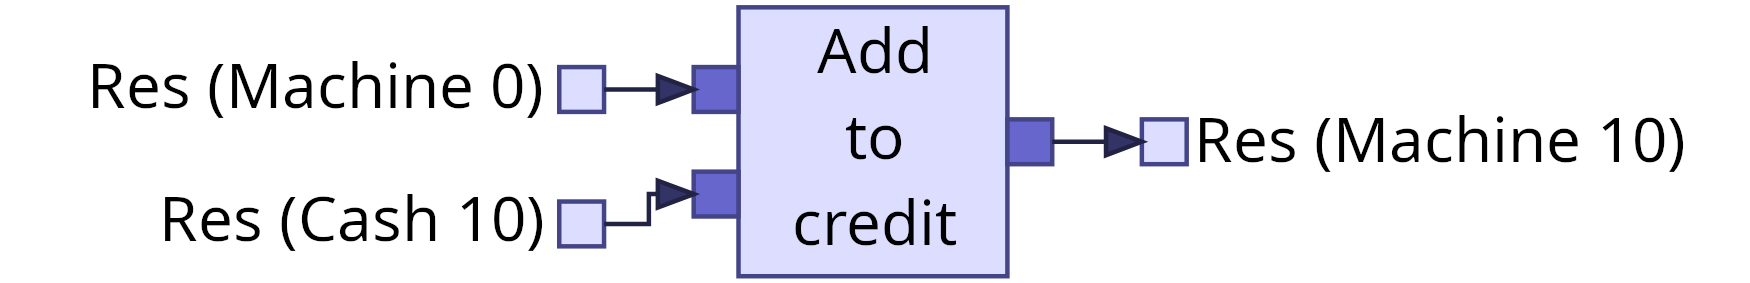
\includegraphics[scale=0.2]{img/add_to_credit_port_graph.png}
  \caption{Port graph \isa{nodePortGraph\ \isalist{}\ \isaString{Add\ to\ credit}\ \isalist{Res\ \isapars{Machine\ 0},\ Res\ \isapars{Cash\ 10}}\ \isalist{Res\ \isapars{Machine\ 10}}}, representing an instance of the \isa{add{\isacharunderscore}to{\isacharunderscore}credit} from Definition~\ref{isa:add_to_credit}.}
  \label{fig:node_port_graph}
\end{figure}

\subsection{Juxtaposition}
\label{sec:port_graphs/mech/par}

Our first complex operation on port graphs is \emph{juxtaposition}, which we will use to represent parallel composition of processes (see Section~\ref{sec:port_graphs/process/constr}).
Informally, it is very simple: take the nodes, edges and open ports of two port graphs and put them into one.
The formal definition, however, needs to be careful about potential clashes when unifying that data.

The first possible clash, and the easiest to solve, is over nodes of the two input port graphs.
We simply assume that the port graphs are disjoint, as characterised by the \isa{pg{\isacharunderscore}disjoint} relation defined in Section~\ref{sec:port_graphs/mech/data}.
To ensure the latter is satisfied before we perform this operation, we can use distinct name atoms to qualify the two port graphs apart (we do so in Section~\ref{sec:port_graphs/process/constr}).

The second possible clash involves the open ports.
Because these ports are identified by their side and the index within, we can avoid the clash by shifting the indices of open ports from one of the input port graphs.
We choose to shift those of the second input, increasing the index of every open port coming from it by the number of open ports on that side coming from the first input.
Since, in a well-formed port graph (see Section~\ref{sec:port_graphs/mech/base_locale}), the number of ports on a side is the upper bound for their index, we know shifting up by that amount will avoid any clash.
Note that this change needs to be done not just in the open ports themselves, but also in any edges that may be adjacent to them.

The last possible clash is with the edges.
However, because edges are pairs of places, which in turn are either ports of nodes or open ports, any potential clashes in them will be taken care of by the adjustments we make to nodes and open ports.

With these considerations in mind, our definition of juxtaposition of port graphs in Isabelle/HOL is as follows:
\begin{isadef}[Juxtaposing port graph]{isa:juxtapose}
  \isacomm{fun}\ juxtapose\ {\isacharcolon}{\isacharcolon}\ {\isachardoublequoteopen}{\isacharparenleft}\isatv{s}\ {\isacharcolon}{\isacharcolon}\ side{\isacharunderscore}in{\isacharunderscore}out{\isacharcomma}\ \isatv{a}{\isacharcomma}\ \isatv{p}{\isacharcomma}\ \isatv{l}{\isacharparenright}\ port{\isacharunderscore}graph\ {\isasymRightarrow}\ {\isacharparenleft}\isatv{s}{\isacharcomma}\ \isatv{a}{\isacharcomma}\ \isatv{p}{\isacharcomma}\ \isatv{l}{\isacharparenright}\ port{\isacharunderscore}graph\isanewline
\isaindent{\isacomm{fun}\ juxtapose\ }{\isasymRightarrow}\ {\isacharparenleft}\isatv{s}{\isacharcomma}\ \isatv{a}{\isacharcomma}\ \isatv{p}{\isacharcomma}\ \isatv{l}{\isacharparenright}\ port{\isacharunderscore}graph{\isachardoublequoteclose}\isanewline
\ \ \isaOcomm{where}\ {\isachardoublequoteopen}\isafv{juxtapose}\ \isabv{x\ y}\ {\isacharequal}\ PGraph\isanewline
\ \ \ \ {\isacharparenleft}\ pg{\isacharunderscore}nodes\ \isabv{x}\ {\isacharat}\ pg{\isacharunderscore}nodes\ \isabv{y}{\isacharparenright}\isanewline
\ \ \ \ {\isacharparenleft}\ pg{\isacharunderscore}edges\ \isabv{x}\ {\isacharat}\isanewline
\ \ \ \ \ \ map\ {\isacharparenleft}shiftOpenInEdge\ {\isacharparenleft}{\isasymlambda}\isabv{s}{\isachardot}\ length\ {\isacharparenleft}filter\ {\isacharparenleft}{\isasymlambda}\isabv{p}{\isachardot}\ port{\isachardot}side\ \isabv{p}\ {\isacharequal}\ \isabv{s}{\isacharparenright}\ {\isacharparenleft}pg{\isacharunderscore}ports\   \isabv{x}{\isacharparenright}{\isacharparenright}{\isacharparenright}\isanewline
\isaindent{\ \ \ \ \ \ map\ {\isacharparenleft}shiftOpenInEdge\ }{\isacharparenleft}{\isasymlambda}\isabv{s}{\isachardot}\ length\ {\isacharparenleft}filter\ {\isacharparenleft}{\isasymlambda}\isabv{p}{\isachardot}\ port{\isachardot}side\ \isabv{p}\ {\isacharequal}\ \isabv{s}{\isacharparenright}\ {\isacharparenleft}pg{\isacharunderscore}ports\   \isabv{x}{\isacharparenright}{\isacharparenright}{\isacharparenright}{\isacharparenright}\isanewline
\isaindent{\ \ \ \ \ \ map\ }{\isacharparenleft}pg{\isacharunderscore}edges\ \isabv{y}{\isacharparenright}{\isacharparenright}\isanewline
\ \ \ \ {\isacharparenleft}\ pg{\isacharunderscore}ports\ \isabv{x}\ {\isacharat}\isanewline
\ \ \ \ \ \ map\ {\isacharparenleft}shiftPort\ {\isacharparenleft}{\isasymlambda}\isabv{s}{\isachardot}\ length\ {\isacharparenleft}filter\ {\isacharparenleft}{\isasymlambda}\isabv{p}{\isachardot}\ port{\isachardot}side\ \isabv{p}\ {\isacharequal}\ \isabv{s}{\isacharparenright}\ {\isacharparenleft}pg{\isacharunderscore}ports\ \isabv{x}{\isacharparenright}{\isacharparenright}{\isacharparenright}{\isacharparenright}\isanewline
\isaindent{\ \ \ \ \ \ map\ }{\isacharparenleft}pg{\isacharunderscore}ports\ \isabv{y}{\isacharparenright}{\isacharparenright}{\isachardoublequoteclose}%

\end{isadef}
\noindent
where \isa{shiftPort} and \isa{shiftOpenInEdge} shift indices of ports, either directly or applying to any open ports contained in an edge.
The amount each port is shifted by is a function of that port's side, allowing for more concise statements.

Figure~\ref{fig:juxtapose} illustrates juxtaposition of two simple port graphs representing primitive actions (see the example introduced in Figure~\ref{fig:node_port_graph}).
The resulting port graph now has three open input ports and three open output ports.
Consider, for instance, the open output port labelled with \isa{Res\ D}.
It starts with index \isa{\isadigit{0}} in its original port graph but has index \isa{\isadigit{1}} after juxtaposition due to the open output port in the other port graph.
In Section~\ref{sec:port_graphs/process/constr}, where we use juxtaposition to represent parallel composition of processes, we also ensure the constituent port graphs are disjoint by qualifying them with distinct name atoms.

\begin{figure}[htbp]
  \centering
  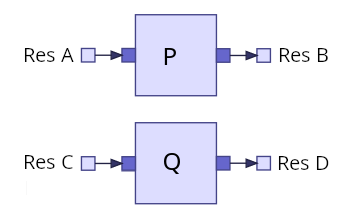
\includegraphics[scale=0.4]{img/par_port_graph_simpler.png}
  \caption{Juxtaposition of two port graphs, which we use to represent parallel composition (see Section~\ref{sec:port_graphs/process/constr}).}
  \label{fig:juxtapose}
\end{figure}

The first property we verify is that this operation preserves the port graph locales we defined.
We state this as the following two theorems, each proven by proving the relevant locale's assumptions:
\begin{isalemma}[Juxtaposition preserves well-formedness]{isa:port_graph_juxtapose}
  \begin{minipage}{0.49\textwidth}
    \isacomm{lemma}\ port{\isacharunderscore}graph{\isacharunderscore}juxtapose{\isacharcolon}\isanewline
\ \ \ \ \isaOcomm{fixes}\ \isafv{x\ y}\ {\isacharcolon}{\isacharcolon}\isanewline
\isaindent{\ \ \ \ \isaOcomm{f}}{\isachardoublequoteopen}{\isacharparenleft}\isatv{s}{\isacharcomma}\ \isatv{a}{\isacharcomma}\ \isatv{p}{\isacharcomma}\ \isatv{l}{\isacharparenright}\ port{\isacharunderscore}graph{\isachardoublequoteclose}\isanewline
\ \ \isaOcomm{assumes}\ {\isachardoublequoteopen}port{\isacharunderscore}graph\ \isafv{x}{\isachardoublequoteclose}\isanewline
\ \ \ \ \ \ \ \ \ \ \isaOcomm{and}\ {\isachardoublequoteopen}port{\isacharunderscore}graph\ \isafv{y}{\isachardoublequoteclose}\isanewline
\ \ \ \ \ \ \ \ \ \ \isaOcomm{and}\ {\isachardoublequoteopen}pg{\isacharunderscore}disjoint\ \isafv{x\ y}{\isachardoublequoteclose}\isanewline
\ \ \ \ \ \ \isaOcomm{shows}\ {\isachardoublequoteopen}port{\isacharunderscore}graph\ {\isacharparenleft}juxtapose\ \isafv{x\ y}{\isacharparenright}{\isachardoublequoteclose}

  \end{minipage}
  \vrule\kern5pt
  \begin{minipage}{0.49\textwidth}
    \isacomm{lemma}\ port{\isacharunderscore}graph{\isacharunderscore}flow{\isacharunderscore}juxtapose{\isacharcolon}\isanewline
\ \ \ \ \isaOcomm{fixes}\ \isafv{x\ y}\ {\isacharcolon}{\isacharcolon}\isanewline
\isaindent{\ \ \ \ \isaOcomm{f}}{\isachardoublequoteopen}{\isacharparenleft}\isatv{s}\ {\isacharcolon}{\isacharcolon}\ side{\isacharunderscore}in{\isacharunderscore}out{\isacharcomma}\ \isatv{a}{\isacharcomma}\ \isatv{p}{\isacharcomma}\ \isatv{l}{\isacharparenright}\ port{\isacharunderscore}graph{\isachardoublequoteclose}\isanewline
\ \ \isaOcomm{assumes}\ {\isachardoublequoteopen}port{\isacharunderscore}graph{\isacharunderscore}flow\ \isafv{x}{\isachardoublequoteclose}\isanewline
\ \ \ \ \ \ \ \ \ \ \isaOcomm{and}\ {\isachardoublequoteopen}port{\isacharunderscore}graph{\isacharunderscore}flow\ \isafv{y}{\isachardoublequoteclose}\isanewline
\ \ \ \ \ \ \ \ \ \ \isaOcomm{and}\ {\isachardoublequoteopen}pg{\isacharunderscore}disjoint\ \isafv{x\ y}{\isachardoublequoteclose}\isanewline
\ \ \ \ \ \ \isaOcomm{shows}\ {\isachardoublequoteopen}port{\isacharunderscore}graph{\isacharunderscore}flow\ {\isacharparenleft}juxtapose\ \isafv{x\ y}{\isacharparenright}{\isachardoublequoteclose}

  \end{minipage}
\end{isalemma}

Next we verify that the operation is associative up to the port graph equivalence.
We prove this according to the definition of port graph equivalence (Definition~\ref{isa:pgEquiv}): both sides are well-formed port graphs with the same set of open ports, and with nodes and edges related by renaming.
By assuming that the corresponding component port graphs are equivalent, we know that there are renaming functions between them.
We use these to form the combined renaming function and show that it relates the nodes and edges correctly.
By assuming that the component port graphs are disjoint, we can determine the source of every node in the two new port graphs and, by extension, the appropriate renaming to apply.
We state the theorem as follows:
\begin{isalemma}[Juxtaposition is associative up to equivalence]{isa:juxtapose_assoc_pgEquiv}
  \isacomm{lemma}\ juxtapose{\isacharunderscore}assoc{\isacharunderscore}pgEquiv{\isacharcolon}\isanewline
\ \ \ \ \ \ \ \ \isaOcomm{fixes}\ \isafv{x\ y\ z}\ {\isacharcolon}{\isacharcolon}\ {\isachardoublequoteopen}{\isacharparenleft}\isatv{s}{\isacharcomma}\ \isatv{a}{\isacharcomma}\ \isatv{p}{\isacharcomma}\ \isatv{l}{\isacharparenright}\ port{\isacharunderscore}graph{\isachardoublequoteclose}\isanewline
\ \ \isaOcomm{assumes}\ {\isachardoublequoteopen}port{\isacharunderscore}graph\ \isafv{x}{\isachardoublequoteclose}\ \isaOcomm{and}\ {\isachardoublequoteopen}port{\isacharunderscore}graph\ \isafv{y}{\isachardoublequoteclose} \isaOcomm{and}\ {\isachardoublequoteopen}port{\isacharunderscore}graph\ \isafv{z}{\isachardoublequoteclose}\isanewline
\ \ \ \ \ \ \ \ \ \ \isaOcomm{and}\ {\isachardoublequoteopen}pg{\isacharunderscore}disjoint\ \isafv{x\ y}{\isachardoublequoteclose}\ \isaOcomm{and}\ {\isachardoublequoteopen}pg{\isacharunderscore}disjoint\ \isafv{y\ z}{\isachardoublequoteclose} \isaOcomm{and}\ {\isachardoublequoteopen}pg{\isacharunderscore}disjoint\ \isafv{x\ z}{\isachardoublequoteclose}\isanewline
\ \ \ \ \ \ \ \ \ \ \isaOcomm{and}\ {\isachardoublequoteopen}port{\isacharunderscore}graph\ \isafv{x{\isacharprime}}{\isachardoublequoteclose}\ \isaOcomm{and}\ {\isachardoublequoteopen}port{\isacharunderscore}graph\ \isafv{y{\isacharprime}}{\isachardoublequoteclose}\ \isaOcomm{and}\ {\isachardoublequoteopen}port{\isacharunderscore}graph\ \isafv{z{\isacharprime}}{\isachardoublequoteclose}\isanewline
\ \ \ \ \ \ \ \ \ \ \isaOcomm{and}\ {\isachardoublequoteopen}pg{\isacharunderscore}disjoint\ \isafv{x{\isacharprime}\ y{\isacharprime}}{\isachardoublequoteclose}\ \isaOcomm{and}\ {\isachardoublequoteopen}pg{\isacharunderscore}disjoint\ \isafv{y{\isacharprime}\ z{\isacharprime}}{\isachardoublequoteclose}\ \isaOcomm{and}\ {\isachardoublequoteopen}pg{\isacharunderscore}disjoint\ \isafv{x{\isacharprime}\ z{\isacharprime}}{\isachardoublequoteclose}\isanewline
\ \ \ \ \ \ \ \ \ \ \isaOcomm{and}\ {\isachardoublequoteopen}\isafv{x}\ {\isasymapprox}\ \isafv{x{\isacharprime}}{\isachardoublequoteclose}\ \isaOcomm{and}\ {\isachardoublequoteopen}\isafv{y}\ {\isasymapprox}\ \isafv{y{\isacharprime}}{\isachardoublequoteclose}\ \isaOcomm{and}\ {\isachardoublequoteopen}\isafv{z}\ {\isasymapprox}\ \isafv{z{\isacharprime}}{\isachardoublequoteclose}\isanewline
\ \ \ \ \ \ \isaOcomm{shows}\ {\isachardoublequoteopen}juxtapose\ {\isacharparenleft}juxtapose\ \isafv{x\ y}{\isacharparenright}\ \isafv{z}\ {\isasymapprox}\ juxtapose\ \isafv{x{\isacharprime}}\ {\isacharparenleft}juxtapose\ \isafv{y{\isacharprime}\ z{\isacharprime}}{\isacharparenright}{\isachardoublequoteclose}

\end{isalemma}

Finally, we verify that juxtapositions of equivalent port graphs are themselves equivalent.
The proof takes the same general form as the associativity proof, being again a proof of equivalence using the same operation, but is rendered simpler by considering fewer port graphs (four instead of six).
We state the theorem as follows:
\begin{isalemma}[Juxtapositions of equivalent port graphs are equivalent]{isa:juxtapose_resp}
  \isacomm{lemma}\ juxtapose{\isacharunderscore}resp{\isacharcolon}\isanewline
\ \ \ \ \ \ \ \ \isaOcomm{fixes}\ \isafv{x\ y}\ {\isacharcolon}{\isacharcolon}\ {\isachardoublequoteopen}{\isacharparenleft}\isatv{s}{\isacharcomma}\ \isatv{a}{\isacharcomma}\ \isatv{p}{\isacharcomma}\ \isatv{l}{\isacharparenright}\ port{\isacharunderscore}graph{\isachardoublequoteclose}\isanewline
\ \ \isaOcomm{assumes}\ {\isachardoublequoteopen}port{\isacharunderscore}graph\ \isafv{x}{\isachardoublequoteclose}\ \isaOcomm{and}\ {\isachardoublequoteopen}port{\isacharunderscore}graph\ \isafv{y}{\isachardoublequoteclose}\ \isaOcomm{and}\ {\isachardoublequoteopen}pg{\isacharunderscore}disjoint\ \isafv{x\ y}{\isachardoublequoteclose}\isanewline
\ \ \ \ \ \ \ \ \ \ \isaOcomm{and}\ {\isachardoublequoteopen}port{\isacharunderscore}graph\ \isafv{x{\isacharprime}}{\isachardoublequoteclose}\ \isaOcomm{and}\ {\isachardoublequoteopen}port{\isacharunderscore}graph\ \isafv{y{\isacharprime}}{\isachardoublequoteclose}\ \isaOcomm{and}\ {\isachardoublequoteopen}pg{\isacharunderscore}disjoint\ \isafv{x{\isacharprime}\ y}{\isacharprime}{\isachardoublequoteclose}\isanewline
\ \ \ \ \ \ \ \ \ \ \isaOcomm{and}\ {\isachardoublequoteopen}\isafv{x}\ {\isasymapprox}\ \isafv{x{\isacharprime}}{\isachardoublequoteclose}\ \isaOcomm{and}\ {\isachardoublequoteopen}\isafv{y}\ {\isasymapprox}\ \isafv{y{\isacharprime}}{\isachardoublequoteclose}\isanewline
\ \ \ \ \ \ \isaOcomm{shows}\ {\isachardoublequoteopen}juxtapose\ \isafv{x\ y}\ {\isasymapprox}\ juxtapose\ \isafv{x{\isacharprime}\ y{\isacharprime}}{\isachardoublequoteclose}

\end{isalemma}

\subsection{Sequencing}
\label{sec:port_graphs/mech/seq}

As our second complex operation on port graphs we define their \emph{sequencing}, which makes use of port graph inputs, outputs and the flow between them.
We use this operation to represent sequential composition of processes (see Section~\ref{sec:port_graphs/process/constr}).
Sequencing goes further than juxtaposition, not just putting the port graphs together but also making new connections and removing other superseded elements.
Informally, on top of combining the port graphs into one, this operation: takes the open output ports of one port graph, matches them with open input ports of the other and ``stitches'' together the edges incident on them.
While doing this, it also applies the same methods for avoiding clashes as juxtaposition (i.e.\ assuming disjoint node names and open port shifting).

The core complexity of this operation is forming the new edges to represent the stitched connection in the result.
For this we define the helper function \isa{seqInterfaceEdges} on the two input port graphs \isa{\isafv{x}} and \isa{\isafv{y}} which:
\begin{enumerate}
  \item Forms a mapping from open output ports of \isa{\isafv{x}} to the edges in \isa{\isafv{x}} going into them.
  \item Forms a mapping from open input ports of \isa{\isafv{y}} to the edges in \isa{\isafv{y}} coming from them.
  \item For each open output port of \isa{\isafv{x}}, uses the mappings to retrieve the edge lists to be stitched: those of \isa{\isafv{x}} going into that port and those of \isa{\isafv{y}} coming from the matching open input port of \isa{\isafv{y}}.
  \item For each such pair of edge lists, form an edge for each combination going from the origin in \isa{\isafv{x}} to the destination in \isa{\isafv{y}}.
\end{enumerate}

The definition of \isa{seqInterfaceEdges} uses the mechanisation of mappings available in Isabelle/HOL, which represents them as functions from a key type to an optional value type.
For the purposes of code generation, this representation can be automatically mapped to a list of key-value pairs.
The full definition is given in Appendix~\ref{app:seqInterfaceEdges}.

\cbstart
In our proofs we mainly interact with this function through two rules: one introducing the fact that an edge is one of its results (Lemma~\ref{isa:seqInterfaceEdges_setI}) and the other decomposing this fact back to its necessary premises (Lemma~\ref{isa:seqInterfaceEdges_setD}).
Both of these tie an edge resulting from \isa{seqInterfaceEdges} to the existence of two edges, one in each input port graph, that ``meet'' at matching open ports and which, when combined, yield that edge.
Note that, since properties we wish to prove (such as the locales in Definition~\ref{isa:locale-port_graph} and Definition~\ref{isa:port_graph_flow}) disregard order of the edges, so do these two rules.
This significantly simplifies them in comparison to the function's implementation with mappings described above.
\cbend

\begin{isalemma}[Introduction rule for elements of \isa{seqInterfaceEdges}]{isa:seqInterfaceEdges_setI}
  \isacomm{lemma}\ seqInterfaceEdges{\isacharunderscore}setI{\isacharcolon}\isanewline
\ \ \ \ \ \ \ \ \isaOcomm{fixes}\ \isafv{x\ y}\ {\isacharcolon}{\isacharcolon}\ {\isachardoublequoteopen}{\isacharparenleft}\isatv{s}\ {\isacharcolon}{\isacharcolon}\ side{\isacharunderscore}in{\isacharunderscore}out{\isacharcomma}\ \isatv{a}{\isacharcomma}\ \isatv{p}{\isacharcomma}\ \isatv{l}{\isacharparenright}\ port{\isacharunderscore}graph{\isachardoublequoteclose}\isanewline
\ \ \isaOcomm{assumes}\ {\isachardoublequoteopen}port{\isacharunderscore}graph{\isacharunderscore}flow\ \isafv{x}{\isachardoublequoteclose}\isanewline
\ \ \ \ \ \ \ \ \ \ \isaOcomm{and}\ {\isachardoublequoteopen}port{\isacharunderscore}graph{\isacharunderscore}flow\ \isafv{y}{\isachardoublequoteclose}\isanewline
\ \ \ \ \ \ \ \ \ \ \isaOcomm{and}\ {\isachardoublequoteopen}edge{\isacharunderscore}from\ \isafv{e}\ {\isacharequal}\ edge{\isacharunderscore}from\ \isafv{a}{\isachardoublequoteclose}\isanewline
\ \ \ \ \ \ \ \ \ \ \isaOcomm{and}\ {\isachardoublequoteopen}\isafv{a}\ {\isasymin}\ set\ {\isacharparenleft}pg{\isacharunderscore}edges\ \isafv{x}{\isacharparenright}{\isachardoublequoteclose}\isanewline
\ \ \ \ \ \ \ \ \ \ \isaOcomm{and}\ {\isachardoublequoteopen}edge{\isacharunderscore}to\ \isafv{e}\ {\isacharequal}\ edge{\isacharunderscore}to\ \isafv{b}{\isachardoublequoteclose}\isanewline
\ \ \ \ \ \ \ \ \ \ \isaOcomm{and}\ {\isachardoublequoteopen}\isafv{b}\ {\isasymin}\ set\ {\isacharparenleft}pg{\isacharunderscore}edges\ \isafv{y}{\isacharparenright}{\isachardoublequoteclose}\isanewline
\ \ \ \ \ \ \ \ \ \ \isaOcomm{and}\ {\isachardoublequoteopen}edge{\isacharunderscore}to\ \isafv{a}\ {\isacharequal}\ OpenPort\ {\isacharparenleft}portSetSide\ Out\ \isafv{p}{\isacharparenright}{\isachardoublequoteclose}\isanewline
\ \ \ \ \ \ \ \ \ \ \isaOcomm{and}\ {\isachardoublequoteopen}edge{\isacharunderscore}from\ \isafv{b}\ {\isacharequal}\ OpenPort\ {\isacharparenleft}portSetSide\ In\ \isafv{p}{\isacharparenright}{\isachardoublequoteclose}\isanewline
\ \ \ \ \ \ \ \ \ \ \isaOcomm{and}\ {\isachardoublequoteopen}port{\isachardot}side\ \isafv{p}\ \isacharequal\ Out{\isachardoublequoteclose}\isanewline
\ \ \ \ \ \ \isaOcomm{shows}\ {\isachardoublequoteopen}\isafv{e}\ {\isasymin}\ set\ {\isacharparenleft}seqInterfaceEdges\ \isafv{x\ y}{\isacharparenright}{\isachardoublequoteclose}

\end{isalemma}
\pagebreak
\begin{isalemma}[Destruction rule for elements of \isa{seqInterfaceEdges}]{isa:seqInterfaceEdges_setD}
  \isacomm{lemma}\ seqInterfaceEdges{\isacharunderscore}setD{\isacharcolon}\isanewline
\ \ \ \ \ \ \ \ \isaOcomm{fixes}\ \isafv{x\ y}\ {\isacharcolon}{\isacharcolon}\ {\isachardoublequoteopen}{\isacharparenleft}\isatv{s}\ {\isacharcolon}{\isacharcolon}\ side{\isacharunderscore}in{\isacharunderscore}out{\isacharcomma}\ \isatv{a}{\isacharcomma}\ \isatv{p}{\isacharcomma}\ \isatv{l}{\isacharparenright}\ port{\isacharunderscore}graph{\isachardoublequoteclose}\isanewline
\ \ \isaOcomm{assumes}\ {\isachardoublequoteopen}\isafv{e}\ {\isasymin}\ set\ {\isacharparenleft}seqInterfaceEdges\ \isafv{x\ y}{\isacharparenright}{\isachardoublequoteclose}\isanewline
\ \ \ \ \isaOcomm{obtains}\ \isafv{a\ b}\ \isaOcomm{and}\ \isafv{p}\ {\isacharcolon}{\isacharcolon}\ {\isachardoublequoteopen}{\isacharparenleft}\isatv{s}{\isacharcomma}\ \isatv{a}{\isacharparenright}\ port{\isachardoublequoteclose}\isanewline
\ \ \ \ \ \ \isaOcomm{where}\ {\isachardoublequoteopen}edge{\isacharunderscore}from\ \isafv{e}\ {\isacharequal}\ edge{\isacharunderscore}from\ \isafv{a}{\isachardoublequoteclose}\isanewline
\ \ \ \ \ \ \ \ \ \ \isaOcomm{and}\ {\isachardoublequoteopen}\isafv{a}\ {\isasymin}\ set\ {\isacharparenleft}pg{\isacharunderscore}edges\ \isafv{x}{\isacharparenright}{\isachardoublequoteclose}\isanewline
\ \ \ \ \ \ \ \ \ \ \isaOcomm{and}\ {\isachardoublequoteopen}edge{\isacharunderscore}to\ \isafv{e}\ {\isacharequal}\ edge{\isacharunderscore}to\ \isafv{b}{\isachardoublequoteclose}\isanewline
\ \ \ \ \ \ \ \ \ \ \isaOcomm{and}\ {\isachardoublequoteopen}\isafv{b}\ {\isasymin}\ set\ {\isacharparenleft}pg{\isacharunderscore}edges\ \isafv{y}{\isacharparenright}{\isachardoublequoteclose}\isanewline
\ \ \ \ \ \ \ \ \ \ \isaOcomm{and}\ {\isachardoublequoteopen}edge{\isacharunderscore}to\ \isafv{a}\ {\isacharequal}\ OpenPort\ {\isacharparenleft}portSetSide\ Out\ \isafv{p}{\isacharparenright}{\isachardoublequoteclose}\isanewline
\ \ \ \ \ \ \ \ \ \ \isaOcomm{and}\ {\isachardoublequoteopen}edge{\isacharunderscore}from\ \isafv{b}\ {\isacharequal}\ OpenPort\ {\isacharparenleft}portSetSide\ In\ \isafv{p}{\isacharparenright}{\isachardoublequoteclose}\isanewline
\ \ \ \ \ \ \ \ \ \ \isaOcomm{and}\ {\isachardoublequoteopen}port{\isachardot}side\ \isafv{p}\ {\isacharequal}\ Out{\isachardoublequoteclose}

\end{isalemma}

With the edges that stitch together the output-input connection, we no longer need the original edges or the open ports used.
To remove the open ports we simply filter them out.
To remove the edges we use the helper function \isa{disconnectFromPlaces~\isafv{ps}~\isafv{es}} which filters the edges \isa{\isafv{es}} to remove any that are incident on a place in \isa{\isafv{ps}}.

\begin{isadef}[Removing edges adjacent on given places]{isa:disconnectFromPlaces}
  \isacomm{definition}\ disconnectFromPlaces\ {\isacharcolon}{\isacharcolon}\ {\isachardoublequoteopen}{\isacharparenleft}\isatv{s}{\isacharcomma}\ \isatv{a}{\isacharcomma}\ \isatv{p}{\isacharparenright}\ place\ list\ {\isasymRightarrow}\ {\isacharparenleft}\isatv{s}{\isacharcomma}\ \isatv{a}{\isacharcomma}\ \isatv{p}{\isacharparenright}\ edge\ list\isanewline
\isaindent{\isacomm{definition}\ disconnectFromPlaces\ }{\isasymRightarrow}\ {\isacharparenleft}\isatv{s}{\isacharcomma}\ \isatv{a}{\isacharcomma}\ \isatv{p}{\isacharparenright}\ edge\ list{\isachardoublequoteclose}\isanewline
\ \ \isaOcomm{where}\ {\isachardoublequoteopen}\isafv{disconnectFromPlaces}\ \isabv{ps\ es}\ {\isacharequal}\isanewline
\ \ \ \ filter\ {\isacharparenleft}{\isasymlambda}\isabv{e}{\isachardot}\ edge{\isacharunderscore}from\ \isabv{e}\ {\isasymnotin}\ set\ \isabv{ps}\ {\isasymand}\ edge{\isacharunderscore}to\ \isabv{e}\ {\isasymnotin}\ set\ \isabv{ps}{\isacharparenright}\ \isabv{es}{\isachardoublequoteclose}

\end{isadef}

Note that these removals need to be taken into account when shifting open ports (and their occurrences in edges) to avoid clashes: one port graph contributes no output and the other contributes no inputs, so only ports on other sides need to be shifted up.

Our definition of port graph sequencing in Isabelle/HOL is shown in Definition~\ref{isa:seqPortGraphs}.
\cbstart
To form the nodes of the result, it simply appends the two lists (line 4).
The edges of the result are split into three groups: first are the new edges forming the connection between the two port graphs (line 5), then the edges of the first port graph except for those that were going to its open outputs (lines 6--8), and finally the edges of the second port graph except for those coming from its open inputs and with the appropriate shifting of indices applied (lines 9--16).
This shifting of indices applies to open ports that are neither inputs nor outputs, and ensures that there can be no clash in open ports coming from the two input port graphs.
Finally, the ports of the result are also split into three groups: all non-output ports of the first port graph (line 17), all output ports of the second port graph (line 18), and all other ports of the second port graph with their indices shifted in the same way (lines 19--20).
\cbend

\begin{isadef}[Sequencing of port graphs]{isa:seqPortGraphs}
  \begin{linenumbers*}
    \isacomm{fun}\ seqPortGraphs\ {\isacharcolon}{\isacharcolon}\ {\isachardoublequoteopen}{\isacharparenleft}\isatv{s}\ {\isacharcolon}{\isacharcolon}\ side{\isacharunderscore}in{\isacharunderscore}out{\isacharcomma}\ \isatv{a}{\isacharcomma}\ \isatv{p}{\isacharcomma}\ \isatv{l}{\isacharparenright}\ port{\isacharunderscore}graph\ {\isasymRightarrow}\ {\isacharparenleft}\isatv{s}{\isacharcomma}\ \isatv{a}{\isacharcomma}\ \isatv{p}{\isacharcomma}\ \isatv{l}{\isacharparenright}\ port{\isacharunderscore}graph\isanewline
\isaindent{\isacomm{fun}\ seqPortGraphs\ }{\isasymRightarrow}\ {\isacharparenleft}\isatv{s}{\isacharcomma}\ \isatv{a}{\isacharcomma}\ \isatv{p}{\isacharcomma}\ \isatv{l}{\isacharparenright}\ port{\isacharunderscore}graph{\isachardoublequoteclose}\isanewline
\ \ \isaOcomm{where}\ {\isachardoublequoteopen}\isafv{seqPortGraphs}\ \isabv{x\ y}\ {\isacharequal}\ PGraph\isanewline
\ \ \ \ {\isacharparenleft}\ pg{\isacharunderscore}nodes\ \isabv{x}\ {\isacharat}\ pg{\isacharunderscore}nodes\ \isabv{y}{\isacharparenright}\isanewline
\ \ \ \ {\isacharparenleft}\ seqInterfaceEdges\ \isabv{x\ y}\ {\isacharat}\isanewline
\ \ \ \ \ \ disconnectFromPlaces\isanewline
\isaindent{\ \ \ \ \ \ di}{\isacharparenleft}map\ OpenPort\ {\isacharparenleft}filter\ {\isacharparenleft}{\isasymlambda}\isabv{x}{\isachardot}\ port{\isachardot}side\ \isabv{x}\ {\isacharequal}\ Out{\isacharparenright}\ {\isacharparenleft}pg{\isacharunderscore}ports\ \isabv{x}{\isacharparenright}{\isacharparenright}{\isacharparenright}\isanewline
\isaindent{\ \ \ \ \ \ di}{\isacharparenleft}pg{\isacharunderscore}edges\ \isabv{x}{\isacharparenright}\ {\isacharat}\isanewline
\ \ \ \ \ \ map\ {\isacharparenleft}shiftOpenInEdge\isanewline
\isaindent{\ \ \ \ \ \ map\ {\isacharparenleft}sh}{\isacharparenleft}{\isasymlambda}\isabv{s}{\isachardot}\ \isanotation{if}\ \isabv{s}\ {\isacharequal}\ In\ {\isasymor}\ \isabv{s}\ {\isacharequal}\ Out\ \isanotation{then}\ {\isadigit{0}}\isanewline
\isaindent{\ \ \ \ \ \ map\ {\isacharparenleft}sh{\isacharparenleft}{\isasymlambda}\isabv{s}{\isachardot}\ }\isanotation{else}\ length\ {\isacharparenleft}filter\ {\isacharparenleft}{\isasymlambda}\isabv{x}{\isachardot}\ port{\isachardot}side\ \isabv{x}\ {\isacharequal}\ \isabv{s}{\isacharparenright}\ {\isacharparenleft}pg{\isacharunderscore}ports\ \isabv{x}{\isacharparenright}{\isacharparenright}{\isacharparenright}\isanewline
\isaindent{\ \ \ \ \ \ map\ {\isacharparenleft}sh}{\isacharparenleft}{\isasymlambda}\isabv{s}{\isachardot}\ \isanotation{if}\ \isabv{s}\ {\isacharequal}\ In\ {\isasymor}\ \isabv{s}\ {\isacharequal}\ Out\ \isanotation{then}\ {\isadigit{0}}\isanewline
\isaindent{\ \ \ \ \ \ map\ {\isacharparenleft}sh{\isacharparenleft}{\isasymlambda}\isabv{s}{\isachardot}\ }\isanotation{else}\ length\ {\isacharparenleft}filter\ {\isacharparenleft}{\isasymlambda}\isabv{x}{\isachardot}\ port{\isachardot}side\ \isabv{x}\ {\isacharequal}\ \isabv{s}{\isacharparenright}\ {\isacharparenleft}pg{\isacharunderscore}ports\ \isabv{x}{\isacharparenright}{\isacharparenright}{\isacharparenright}{\isacharparenright}\isanewline
\isaindent{\ \ \ \ \ \ map\ }{\isacharparenleft}disconnectFromPlaces\isanewline
\isaindent{\ \ \ \ \ \ map\ {\isacharparenleft}di}{\isacharparenleft}map\ OpenPort\ {\isacharparenleft}filter\ {\isacharparenleft}{\isasymlambda}\isabv{x}{\isachardot}\ port{\isachardot}side\ \isabv{x}\ {\isacharequal}\ In{\isacharparenright}\ {\isacharparenleft}pg{\isacharunderscore}ports\ \isabv{y}{\isacharparenright}{\isacharparenright}{\isacharparenright}\isanewline
\isaindent{\ \ \ \ \ \ map\ {\isacharparenleft}di}{\isacharparenleft}pg{\isacharunderscore}edges\ \isabv{y}{\isacharparenright}{\isacharparenright}{\isacharparenright}\isanewline
\ \ \ \ {\isacharparenleft}\ filter\ {\isacharparenleft}{\isasymlambda}\isabv{x}{\isachardot}\ port{\isachardot}side\ \isabv{x}\ {\isasymnoteq}\ Out{\isacharparenright}\ {\isacharparenleft}pg{\isacharunderscore}ports\ \isabv{x}{\isacharparenright}\ {\isacharat}\isanewline
\ \ \ \ \ \ filter\ {\isacharparenleft}{\isasymlambda}\isabv{x}{\isachardot}\ port{\isachardot}side\ \isabv{x}\ {\isacharequal}\ Out{\isacharparenright}\ {\isacharparenleft}pg{\isacharunderscore}ports\ \isabv{y}{\isacharparenright}\ {\isacharat}\isanewline
\ \ \ \ \ \ map\ {\isacharparenleft}shiftPort\ {\isacharparenleft}{\isasymlambda}\isabv{s}{\isachardot}\ length\ {\isacharparenleft}filter\ {\isacharparenleft}{\isasymlambda}\isabv{p}{\isachardot}\ port{\isachardot}side\ \isabv{p}\ {\isacharequal}\ \isabv{s}{\isacharparenright}\ {\isacharparenleft}pg{\isacharunderscore}ports\ \isabv{x}{\isacharparenright}{\isacharparenright}{\isacharparenright}{\isacharparenright}\isanewline
\ \ \ \ \ \ \isaindent{map}\ {\isacharparenleft}filter\ {\isacharparenleft}{\isasymlambda}\isabv{x}{\isachardot}\ port{\isachardot}side\ \isabv{x}\ {\isasymnoteq}\ In\ {\isasymand}\ port{\isachardot}side\ \isabv{x}\ {\isasymnoteq}\ Out{\isacharparenright}\ {\isacharparenleft}pg{\isacharunderscore}ports\ \isabv{y}{\isacharparenright}{\isacharparenright}{\isacharparenright}{\isachardoublequoteclose}%

  \end{linenumbers*}
\end{isadef}

Figure~\ref{fig:seqPortGraphs} illustrates sequencing of the same simple port graphs as our example of juxtaposition in Figure~\ref{fig:juxtapose}.
The resulting port graph now only has one open input port and one open output port.
The open ports labelled \isa{Res\ B} and \isa{Res\ C} in the original port graphs are stitched together by \isa{seqInterfaceEdges} to form two edges between ground ports instead.
As with juxtaposition, in Section~\ref{sec:port_graphs/process/constr} we qualify the constituent port graphs to ensure they are disjoint.

\begin{figure}[htb]
  \centering
  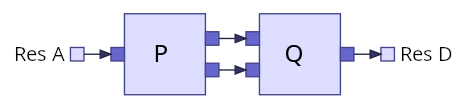
\includegraphics[scale=0.4]{img/seq_port_graph.png}
  \caption{Sequencing of two port graphs, which we use to represent sequential composition (see Section~\ref{sec:port_graphs/process/constr}).}
  \label{fig:seqPortGraphs}
\end{figure}

Once again, the first property we verify is that this operation preserves the port graph locales.
In this case, however, even proving that the base locale remain satisfied requires facts from the flow locale.
For instance, if an edge is part of the stitched connection, then its origin is only guaranteed to be in the port graph because we know it could not have been one of the open output ports that were removed.
More complex situations requiring facts about the flow arise as part of proving that this process does not introduce any duplicate edges.
As such, we state this as a single theorem, albeit in almost the same form as the one for juxtaposition:
\begin{isalemma}[Sequencing port graphs preserves well-formedness]{isa:port_graph_flow_seqPortGraphs}
  \isacomm{lemma}\ port{\isacharunderscore}graph{\isacharunderscore}flow{\isacharunderscore}seqPortGraphs{\isacharcolon}\isanewline
\ \ \ \ \ \ \ \ \isaOcomm{fixes}\ \isafv{x\ y}\ {\isacharcolon}{\isacharcolon}\ {\isachardoublequoteopen}{\isacharparenleft}\isatv{s}\ {\isacharcolon}{\isacharcolon}\ side{\isacharunderscore}in{\isacharunderscore}out{\isacharcomma}\ \isatv{a}{\isacharcomma}\ \isatv{p}{\isacharcomma}\ \isatv{l}{\isacharparenright}\ port{\isacharunderscore}graph{\isachardoublequoteclose}\isanewline
\ \ \isaOcomm{assumes}\ {\isachardoublequoteopen}port{\isacharunderscore}graph{\isacharunderscore}flow\ \isafv{x}{\isachardoublequoteclose}\isanewline
\ \ \ \ \ \ \ \ \ \ \isaOcomm{and}\ {\isachardoublequoteopen}port{\isacharunderscore}graph{\isacharunderscore}flow\ \isafv{y}{\isachardoublequoteclose}\isanewline
\ \ \ \ \ \ \ \ \ \ \isaOcomm{and}\ {\isachardoublequoteopen}pg{\isacharunderscore}disjoint\ \isafv{x\ y}{\isachardoublequoteclose}\isanewline
\ \ \ \ \ \ \isaOcomm{shows}\ {\isachardoublequoteopen}port{\isacharunderscore}graph{\isacharunderscore}flow\ {\isacharparenleft}seqPortGraphs\ \isafv{x\ y}{\isacharparenright}{\isachardoublequoteclose}

\end{isalemma}

The other two properties, namely that the operation is associative and respects port graph equivalence, are stated in the same form as those for juxtaposition except for the port graphs needing to satisfy the stronger \isa{port{\isacharunderscore}graph{\isacharunderscore}flow} locale.
It is the proofs of these properties that are made more complex due to the operation being more complex.
For instance, when proving that edges of the two resulting port graphs are related by renaming, we need to consider more cases: an edge could come from any of the constituent port graphs or be the result of one of the stitched interfaces.
In each case we need to find the corresponding edge in the other resulting port graph and show that the combined renaming function indeed relates them.
\begin{isalemma}[Sequencing is associative up to equivalence]{isa:seqPortGraphs_assoc_pgEquiv}
  \isacomm{lemma}\ seqPortGraphs{\isacharunderscore}assoc{\isacharunderscore}pgEquiv{\isacharcolon}\isanewline
\ \ \ \ \ \ \ \ \isaOcomm{fixes}\ \isafv{x\ y\ z}\ {\isacharcolon}{\isacharcolon}\ {\isachardoublequoteopen}{\isacharparenleft}\isatv{s}\ {\isacharcolon}{\isacharcolon}\ side{\isacharunderscore}in{\isacharunderscore}out{\isacharcomma}\ \isatv{a}{\isacharcomma}\ \isatv{p}{\isacharcomma}\ \isatv{l}{\isacharparenright}\ port{\isacharunderscore}graph{\isachardoublequoteclose}\isanewline
\ \ \isaOcomm{assumes}\ {\isachardoublequoteopen}port{\isacharunderscore}graph{\isacharunderscore}flow\ \isafv{x}{\isachardoublequoteclose}\ \isaOcomm{and}\ {\isachardoublequoteopen}port{\isacharunderscore}graph{\isacharunderscore}flow\ \isafv{y}{\isachardoublequoteclose} \isaOcomm{and}\ {\isachardoublequoteopen}port{\isacharunderscore}graph{\isacharunderscore}flow\ \isafv{z}{\isachardoublequoteclose}\isanewline
\ \ \ \ \ \ \ \ \ \ \isaOcomm{and}\ {\isachardoublequoteopen}pg{\isacharunderscore}disjoint\ \isafv{x\ y}{\isachardoublequoteclose}\ \isaOcomm{and}\ {\isachardoublequoteopen}pg{\isacharunderscore}disjoint\ \isafv{y\ z}{\isachardoublequoteclose} \isaOcomm{and}\ {\isachardoublequoteopen}pg{\isacharunderscore}disjoint\ \isafv{x\ z}{\isachardoublequoteclose}\isanewline
\ \ \ \ \ \ \ \ \ \ \isaOcomm{and}\ {\isachardoublequoteopen}port{\isacharunderscore}graph{\isacharunderscore}flow\ \isafv{x{\isacharprime}}{\isachardoublequoteclose}\ \isaOcomm{and}\ {\isachardoublequoteopen}port{\isacharunderscore}graph{\isacharunderscore}flow\ \isafv{y{\isacharprime}}{\isachardoublequoteclose}\ \isaOcomm{and}\ {\isachardoublequoteopen}port{\isacharunderscore}graph{\isacharunderscore}flow\ \isafv{z{\isacharprime}}{\isachardoublequoteclose}\isanewline
\ \ \ \ \ \ \ \ \ \ \isaOcomm{and}\ {\isachardoublequoteopen}pg{\isacharunderscore}disjoint\ \isafv{x{\isacharprime}\ y{\isacharprime}}{\isachardoublequoteclose}\ \isaOcomm{and}\ {\isachardoublequoteopen}pg{\isacharunderscore}disjoint\ \isafv{y{\isacharprime}\ z{\isacharprime}}{\isachardoublequoteclose}\ \isaOcomm{and}\ {\isachardoublequoteopen}pg{\isacharunderscore}disjoint\ \isafv{x{\isacharprime}\ z{\isacharprime}}{\isachardoublequoteclose}\isanewline
\ \ \ \ \ \ \ \ \ \ \isaOcomm{and}\ {\isachardoublequoteopen}\isafv{x}\ {\isasymapprox}\ \isafv{x{\isacharprime}}{\isachardoublequoteclose}\ \isaOcomm{and}\ {\isachardoublequoteopen}\isafv{y}\ {\isasymapprox}\ \isafv{y{\isacharprime}}{\isachardoublequoteclose}\ \isaOcomm{and}\ {\isachardoublequoteopen}\isafv{z}\ {\isasymapprox}\ \isafv{z{\isacharprime}}{\isachardoublequoteclose}\isanewline
\ \ \ \ \ \ \isaOcomm{shows}\ {\isachardoublequoteopen}seqPortGraphs\ {\isacharparenleft}seqPortGraphs\ \isafv{x\ y}{\isacharparenright}\ \isafv{z}\ {\isasymapprox}\isanewline
\isaindent{\ \ \ \ \ \ \isaOcomm{shows}\ {\isachardoublequoteopen}}seqPortGraphs\ \isafv{x{\isacharprime}}\ {\isacharparenleft}seqPortGraphs\ \isafv{y{\isacharprime}\ z{\isacharprime}}{\isacharparenright}{\isachardoublequoteclose}

\end{isalemma}
\begin{isalemma}[Sequencings of equivalent port graphs are equivalent]{isa:seqPortGraphs_resp}
  \isacomm{lemma}\ seqPortGraphs{\isacharunderscore}resp{\isacharcolon}\isanewline
\ \ \ \ \ \ \ \ \isaOcomm{fixes}\ \isafv{x\ y}\ {\isacharcolon}{\isacharcolon}\ {\isachardoublequoteopen}{\isacharparenleft}\isatv{s}\ {\isacharcolon}{\isacharcolon}\ side{\isacharunderscore}in{\isacharunderscore}out{\isacharcomma}\ \isatv{a}{\isacharcomma}\ \isatv{p}{\isacharcomma}\ \isatv{l}{\isacharparenright}\ port{\isacharunderscore}graph{\isachardoublequoteclose}\isanewline
\ \ \isaOcomm{assumes}\ {\isachardoublequoteopen}port{\isacharunderscore}graph{\isacharunderscore}flow\ \isafv{x}{\isachardoublequoteclose}\ \isaOcomm{and}\ {\isachardoublequoteopen}port{\isacharunderscore}graph{\isacharunderscore}flow\ \isafv{y}{\isachardoublequoteclose}\ \isaOcomm{and}\ {\isachardoublequoteopen}pg{\isacharunderscore}disjoint\ \isafv{x\ y}{\isachardoublequoteclose}\isanewline
\ \ \ \ \ \ \ \ \ \ \isaOcomm{and}\ {\isachardoublequoteopen}port{\isacharunderscore}graph{\isacharunderscore}flow\ \isafv{x{\isacharprime}}{\isachardoublequoteclose}\ \isaOcomm{and}\ {\isachardoublequoteopen}port{\isacharunderscore}graph{\isacharunderscore}flow\ \isafv{y{\isacharprime}}{\isachardoublequoteclose}\ \isaOcomm{and}\ {\isachardoublequoteopen}pg{\isacharunderscore}disjoint\ \isafv{x{\isacharprime}\ y}{\isacharprime}{\isachardoublequoteclose}\isanewline
\ \ \ \ \ \ \ \ \ \ \isaOcomm{and}\ {\isachardoublequoteopen}\isafv{x}\ {\isasymapprox}\ \isafv{x{\isacharprime}}{\isachardoublequoteclose}\ \isaOcomm{and}\ {\isachardoublequoteopen}\isafv{y}\ {\isasymapprox}\ \isafv{y{\isacharprime}}{\isachardoublequoteclose}\isanewline
\ \ \ \ \ \ \isaOcomm{shows}\ {\isachardoublequoteopen}seqPortGraphs\ \isafv{x\ y}\ {\isasymapprox}\ seqPortGraphs\ \isafv{x{\isacharprime}\ y{\isacharprime}}{\isachardoublequoteclose}

\end{isalemma}

\subsection{Port Graph Export}
\label{sec:port_graphs/mech/export}

Our mechanisation allows us to specify concrete port graphs, manipulate them and prove their properties.
However, being firmly in the algebraic environment of Isabelle, we cannot directly visualise them.
That means we miss out on a significant advantage offered by their graphical nature to human comprehension.

Outside the proof assistant there exist tools which, given the data describing a port graph, lay the individual elements out on a plane and turn it into an image.
We take advantage of this by mechanising a function from port graphs to the data such a tool needs.

We target the Eclipse Layout Kernel (ELK)~\cite{domros_et_al-2023}, which can represent (hierarchical) port graphs and implements a range of graph layout algorithms, and Eclipse Sprotty~\footnote{\url{https://projects.eclipse.org/projects/ecd.sprotty}}, which is a web-based diagramming framework compatible with ELK.
Their integration is shown by the online ELK Demonstrators~\footnote{\url{https://rtsys.informatik.uni-kiel.de/elklive/}}.

Within Isabelle/HOL, we use the existing mechanisation of JSON due to Brucker~\cite{Nano_JSON-AFP} to define a function from port graphs into an ELK-compatible JSON object.
While most of the implementation (given in full in Appendix~\ref{app:elk_export}) consists of directly turning each aspect of our port graphs into the ELK JSON counterpart, we also need to convert the type variables port graphs use into a form comprehensible to ELK.
As such, we parameterise the conversion function with the following domain-dependent functions:
\begin{itemize}
  \item Mapping of port graph sides to the five port sides that ELK supports: \texttt{UNDEFINED}, \texttt{NORTH}, \texttt{EAST}, \texttt{SOUTH}, \texttt{WEST}.
    For instance, with process port graphs we map \isa{In} to \texttt{WEST} and \isa{Out} to \texttt{EAST}.
  \item Mapping of node names to string literals, so they can be used as components in unique identifiers.
    For instance, with process port graphs we simply print the path to the relevant action in the composition tree to uniquely identify it.
  \item Mapping of node labels to string literals, so they can be used as node labels in the visualisation.
    For instance, with process port graphs we use the action's label.
\end{itemize}

Once instantiated for a specific type of port graphs, such as process port graphs, the conversion function produces formal JSON objects.
These we then turn into text and visualise using the online ELK JSON Demonstrator~\footnote{\url{https://rtsys.informatik.uni-kiel.de/elklive/json.html}}.
We use this method to visualise the port graphs in the present chapter, but in Section~\ref{sec:port_graphs/conc} we note the potential for a more closely tailored tool.

\subsection{Summary}

We have mechanised a self-contained theory of port graphs, which we will use in the following sections to graphically reason about process compositions.
It includes the data representing port graphs, constraints on that data and two significant port graph compositions.

While certainly influenced by our intention, we believe this theory is sufficiently general to be of use for formal verification in other contexts.
As noted in Section~\ref{sec:port_graphs/rel}, port graphs have been used to model biochemical processes and social networks, and are connected to graphical languages used, for instance, to reason about quantum circuits.

In the next section we specialise this general theory to our case of graphical representation of process compositions and use the language of port graphs to prove their various properties.
This perspective is particularly useful when talking about resource connections between actions.

\section{Process Port Graphs}
\label{sec:port_graphs/process}

Turning process compositions into port graphs, we use nodes to represent primitive actions and edges to represent the resource connections between those actions.
These resource connections are the result of composition operations and resource actions, which we represent with port graph operations and node-less port graphs respectively.

\cbstart
Note that with process port graphs we can use the tools described in Section~\ref{sec:port_graphs/mech/export} to visualise process compositions.
This differs in several ways from the process diagrams of Section~\ref{sec:proc/diag}.
First, as discussed in more detail in Section~\ref{sec:port_graphs/process/constr}, our construction only applies to a subset of process compositions while the process diagrams apply to all valid compositions.
However, second, the process port graphs tie compositions \emph{formally} to the graphical representation, allowing us to prove their properties, while process diagrams are informal.
Third, where both visualisations exist they will often differ in their layout, since the layout of port graphs is determined by an algorithm based on the present connections while the layout of process diagrams is determined na\"{i}vely from the composition structure.
But the connections between actions that both visualisations represent will be the same.
\cbend

We start this section by discussion of how we specialise the general type of port graphs to suit our purposes.
Then we describe the translation itself and continue on to its verified properties.
In the following section we will discuss our main theorem stemming from this translation, a graphical proof of process linearity.

\subsection{Preliminaries}
\label{sec:port_graphs/process/prelim}

Before we can even state how process compositions relate to port graphs, we need to instantiate the type variables of port graphs to specify the sides, name atoms, node labels and port labels.
We give these instantiations relative to the process composition type variables: \isa{\isatv{a}} and \isa{\isatv{b}} for linear and copyable resource atoms respectively, and \isa{\isatv{l}} and \isa{\isatv{m}} for primitive process label and metadata respectively.
\cbar{Note that, with regards to ports, the instantiation matches that of Section~\ref{sec:proc/diag/paths} for process diagrams.}

To represent process compositions we only need two sides: input and output.
\cbar{We reuse our formalisation of these sides from Section~\ref{sec:proc/diag/paths} and prove it} to be an instance of the \isa{side{\isacharunderscore}in{\isacharunderscore}out} type class from Section~\ref{sec:port_graphs/mech/flow_locale}.
\begin{isadef}[Datatype of process sides, an instance of \isa{side{\isacharunderscore}in{\isacharunderscore}out}]{isa:process_side}
  \isacomm{datatype}\ process{\isacharunderscore}side\ \isacharequal\ In\ \isacharbar\ Out

\item
  \isacomm{instantiation}\ process{\isacharunderscore}side\ \ty\ side{\isacharunderscore}in{\isacharunderscore}out\isanewline
\isaOcomm{begin}\isanewline
\ \ \isacomm{definition}\ In\ \isacharequal\ process{\isacharunderscore}side{\isachardot}In\isanewline
\ \ \isacomm{definition}\ Out\ \isacharequal\ process{\isacharunderscore}side{\isachardot}Out\isanewline
\ \ \isacomm{instance\ by}\ standard\ \isapars{simp\ \quasi{add:}\ In{\isacharunderscore}process{\isacharunderscore}side{\isacharunderscore}def\ Out{\isacharunderscore}process{\isacharunderscore}side{\isacharunderscore}def}\isanewline
\isaOcomm{end}

\end{isadef}

Nodes in this case represent primitive actions, which can be uniquely identified in a process composition by the path to that leaf.
See Section~\ref{sec:proc/diag/paths} for our earlier discussion of these paths and their formalisation, which we reuse here (reproduced in Definition~\ref{isa:process_inner-again}.
As such, the name atoms we use are the type \isa{process{\isacharunderscore}inner}.
\begin{isadef}[Components for composition tree paths]{isa:process_inner-again}
  \isacomm{datatype}\ process{\isacharunderscore}inner\ {\isacharequal}\ SeqL\ {\isacharbar}\ SeqR\ {\isacharbar}\ ParL\ {\isacharbar}\ ParR\ {\isacharbar}\ OptL\ {\isacharbar}\ OptR\ {\isacharbar}\ Rep

\end{isadef}

Furthermore, because the only nodes are primitive actions, we annotate them with the extra data of those actions.
For this we define a new datatype, \isa{\isapars{\isatv{l}{\isacharcomma}\ \isatv{m}}\ node{\isacharunderscore}content}, to collect together an action's label and metadata:
\begin{isadef}[Datatype holding node content]{isa:node_content}
  \isacomm{datatype}\ \isapars{\isatv{l}{\isacharcomma}\ \isatv{m}}\ node{\isacharunderscore}content\ \isacharequal\ NodePrimitive\ \isapars{\isatv{l}}\ \isapars{\isatv{m}}

\end{isadef}

Ports represent parallel parts of the input and output resources of an action, so we annotate them with the relevant resources.
\cbar{See our discussion of ports in the context of} process diagrams in Section~\ref{sec:proc/diag/paths}.
As such, the port labels we use are the type \isa{\isapars{\isatv{a}{\isacharcomma}\ \isatv{b}}\ resource}.

All together, the specific type of port graphs we use is the following:
\begin{isabelle}
\centering
  {\isacharparenleft}process{\isacharunderscore}side{\isacharcomma}\ {\isacharparenleft}\isatv{a}{\isacharcomma}\ \isatv{b}{\isacharparenright}\ resource{\isacharcomma}\ process{\isacharunderscore}inner{\isacharcomma}\ {\isacharparenleft}\isatv{l}{\isacharcomma}\ \isatv{m}{\isacharparenright}\ node{\isacharunderscore}content{\isacharparenright}\ port{\isacharunderscore}graph
\end{isabelle}
which we abbreviate as:
\begin{isabelle}
\centering
  {\isacharparenleft}\isatv{a}{\isacharcomma}\ \isatv{b}{\isacharcomma}\ \isatv{l}{\isacharcomma}\ \isatv{m}{\isacharparenright}\ process{\isacharunderscore}port{\isacharunderscore}graph
\end{isabelle}

\subsection{Process Port Graph Construction}
\label{sec:port_graphs/process/constr}

We construct port graphs from processes by associating each action with a port graph template and each composition operation with an operation on port graphs, as shown in Definition~\ref{isa:pgConstruct}.
\cbar{We follow it with more detailed discussion of its cases.}

\begin{isadef}[Constructing a port graph from a process composition]{isa:pgConstruct}
  \isacomm{primrec}\ pgConstruct\ {\isacharcolon}{\isacharcolon}\ {\isachardoublequoteopen}{\isacharparenleft}\isatv{a}{\isacharcomma}\ \isatv{b}{\isacharcomma}\ \isatv{l}{\isacharcomma}\ \isatv{m}{\isacharparenright}\ process\ {\isasymRightarrow}\ {\isacharparenleft}\isatv{a}{\isacharcomma}\ \isatv{b}{\isacharcomma}\ \isatv{l}{\isacharcomma}\ \isatv{m}{\isacharparenright}\ process{\isacharunderscore}port{\isacharunderscore}graph{\isachardoublequoteclose}\isanewline
\ \ \isaOcomm{where}\isanewline
\ \ \ \ {\isachardoublequoteopen}\isafv{pgConstruct}\ {\isacharparenleft}Primitive\ \isabv{ins\ outs\ l\ m}{\isacharparenright}\ {\isacharequal}\isanewline
\ \ \ \ nodePortGraph\ {\isacharbrackleft}{\isacharbrackright}\ {\isacharparenleft}NodePrimitive\ \isabv{l\ m}{\isacharparenright}\ {\isacharparenleft}parallel{\isacharunderscore}parts\ \isabv{ins}{\isacharparenright}\ {\isacharparenleft}parallel{\isacharunderscore}parts\ \isabv{outs}{\isacharparenright}{\isachardoublequoteclose}\isanewline
\ \ {\isacharbar}\ {\isachardoublequoteopen}\isafv{pgConstruct}\ {\isacharparenleft}Seq\ \isabv{p\ q}{\isacharparenright}\ {\isacharequal}\isanewline
\ \ \ \ seqPortGraphs\ {\isacharparenleft}qualifyPortGraph\ SeqL\ {\isacharparenleft}\isafv{pgConstruct}\ \isabv{p}{\isacharparenright}{\isacharparenright}\isanewline
\isaindent{\ \ \ \ seqPortGraphs\ }{\isacharparenleft}qualifyPortGraph\ SeqR\ {\isacharparenleft}\isafv{pgConstruct}\ \isabv{q}{\isacharparenright}{\isacharparenright}{\isachardoublequoteclose}\isanewline
\ \ {\isacharbar}\ {\isachardoublequoteopen}\isafv{pgConstruct}\ {\isacharparenleft}Par\ \isabv{p\ q}{\isacharparenright}\ {\isacharequal}\isanewline
\ \ \ \ juxtapose\ {\isacharparenleft}qualifyPortGraph\ ParL\ {\isacharparenleft}\isafv{pgConstruct}\ \isabv{p}{\isacharparenright}{\isacharparenright}\isanewline
\isaindent{\ \ \ \ juxtapose\ }{\isacharparenleft}qualifyPortGraph\ ParR\ {\isacharparenleft}\isafv{pgConstruct}\ \isabv{q}{\isacharparenright}{\isacharparenright}{\isachardoublequoteclose}\isanewline
\ \ {\isacharbar}\ {\isachardoublequoteopen}\isafv{pgConstruct}\ {\isacharparenleft}Identity\ \isabv{a}{\isacharparenright}\ {\isacharequal}\ idPortGraph\ {\isacharparenleft}parallel{\isacharunderscore}parts\ \isabv{a}{\isacharparenright}{\isachardoublequoteclose}\isanewline
\ \ {\isacharbar}\ {\isachardoublequoteopen}\isafv{pgConstruct}\ {\isacharparenleft}Swap\ \isabv{a\ b}{\isacharparenright}\ {\isacharequal}\ swapPortGraph\ {\isacharparenleft}parallel{\isacharunderscore}parts\ \isabv{a}{\isacharparenright}\ {\isacharparenleft}parallel{\isacharunderscore}parts\ \isabv{b}{\isacharparenright}{\isachardoublequoteclose}\isanewline
\ \ {\isacharbar}\ {\isachardoublequoteopen}\isafv{pgConstruct}\ {\isacharparenleft}Duplicate\ \isabv{a}{\isacharparenright}\ {\isacharequal}\ forkPortGraph\ {\isacharparenleft}Copyable\ \isabv{a}{\isacharparenright}{\isachardoublequoteclose}\isanewline
\ \ {\isacharbar}\ {\isachardoublequoteopen}\isafv{pgConstruct}\ {\isacharparenleft}Erase\ \isabv{a}{\isacharparenright}\ {\isacharequal}\ endPortGraph\ {\isacharbrackleft}Copyable\ \isabv{a}{\isacharbrackright}{\isachardoublequoteclose}\isanewline
\ \ {\isacharbar}\ {\isachardoublequoteopen}\isafv{pgConstruct}\ {\isacharparenleft}Repeat\ \isabv{a\ b}{\isacharparenright}\ {\isacharequal}\ forkPortGraph\ {\isacharparenleft}Repeatable\ \isabv{a\ b}{\isacharparenright}{\isachardoublequoteclose}\isanewline
\ \ {\isacharbar}\ {\isachardoublequoteopen}\isafv{pgConstruct}\ {\isacharparenleft}Close\ \isabv{a\ b}{\isacharparenright}\ {\isacharequal}\ endPortGraph\ {\isacharbrackleft}Repeatable\ \isabv{a\ b}{\isacharbrackright}{\isachardoublequoteclose}\isanewline
\ \ {\isacharbar}\ {\isachardoublequoteopen}\isafv{pgConstruct}\ {\isacharparenleft}Once\ \isabv{a\ b}{\isacharparenright}\ {\isacharequal}\ oncePortGraph\ \isabv{a\ b}{\isachardoublequoteclose}\isanewline
\ \ {\isacharbar}\ {\isachardoublequoteopen}\isafv{pgConstruct}\ {\isacharparenleft}Forget\ \isabv{a}{\isacharparenright}\ {\isacharequal}\ forgetPortGraph\ \isabv{a}{\isachardoublequoteclose}%

\end{isadef}

Note that we provide no definitions for the non-deterministic and higher-order cases, as those cannot be captured faithfully by our present theory of port graphs.
\cbar{While we use port indices to represent parallel resources, a more complicated approach would be needed to also represent non-deterministic combinations of resources in a way that works well with optional composition and the relevant resource actions.
For instance, we may want the graphical representation of an injection action followed by optional composition to result in just the corresponding branch of the composition being reachable.
In the case of representing a composition as a repeatable executable resource, we would need at least hierarchical port graphs to allow nodes to contain whole port graphs.
As such, expanding the construction to all compositions is part of future work, as described in Section~\ref{sec:port_graphs/conc}).}

In the primitive action case, we make use of the simple single-node port graph previously discussed in Section~\ref{sec:port_graphs/mech/simple-ex} and shown again in Figure~\ref{fig:primitive_port_graph}.
Because this action by itself is the root of its own composition tree, we use the empty name \isa{\isalist{}} for the node.
The label we give it is the action's label and metadata, while the input and output port data lists are the parallel parts of the input and output resources.

\begin{figure}[htbp]
  \centering
  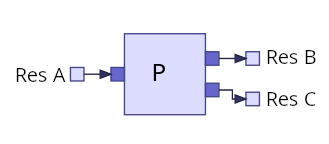
\includegraphics[scale=0.5]{img/node_port_graph.png}
  \caption{Port graph \isa{Primitive\ \isapars{Res\ A}\ \isapars{Res\ B\ \isasymodot\ Res\ C}\ \isaString{P}\ \isapars{}}}
  \label{fig:primitive_port_graph}
\end{figure}

For the sequential and parallel composition cases, we make use of the port graph sequencing (see Section~\ref{sec:port_graphs/mech/seq}) and juxtaposition (see Section~\ref{sec:port_graphs/mech/par}) respectively.
We first recursively construct the port graphs of the child processes and qualify them with distinct name atoms to prevent an overlap in the names they contain.
Then we apply the relevant operation to the resulting port graphs, which takes care of all other aspects given disjoint port graphs.
Instances for two primitive actions composed in sequence and in parallel are shown in Figure~\ref{fig:seq_par_port_graph}.

\begin{figure}[htbp]
  \begin{subfigure}{0.45\textwidth}
    \centering
    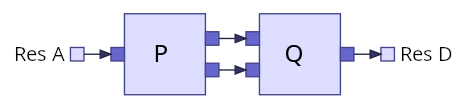
\includegraphics[scale=0.4]{img/seq_port_graph.png}
    \caption{Sequential composition}
    \label{fig:seq_port_graph}
  \end{subfigure}
  \begin{subfigure}{0.45\textwidth}
    \centering
    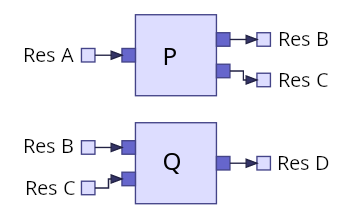
\includegraphics[scale=0.4]{img/par_port_graph.png}
    \caption{Parallel composition}
    \label{fig:par_port_graph}
  \end{subfigure}
  \caption{Process port graphs for sequential and parallel composition of primitive actions \isa{P:\ Res\ A\ \isasymrightarrow\ Res\ B\ \isasymodot\ Res\ C} and \isa{Q:\ Res\ B\ \isasymodot\ Res\ C\ \isasymrightarrow\ Res\ D}}
  \label{fig:seq_par_port_graph}
\end{figure}

For \isa{Identity} we build a port graph consisting of no node and a set of edges, one for each parallel part of the relevant resource going between two open ports, one input and one output.
We abstract this pattern in general port graphs for any list of data (in our case the parallel parts of a resource) and call it \isa{idPortGraph}.
Its instance for the three-atom resource \isa{Res\ A\ \isasymodot\ Res\ B\ \isasymodot\ Res\ C} is shown in Figure~\ref{fig:id_port_graph}.

\begin{figure}[htbp]
  \centering
  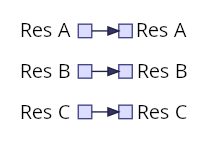
\includegraphics[scale=0.5]{img/id_port_graph.png}
  \caption{Process port graph for \isa{Identity\ \isapars{Res\ A\ \isasymodot\ Res\ B\ \isasymodot\ Res\ C}}}
  \label{fig:id_port_graph}
\end{figure}

For \isa{Swap} we build again a port graph consisting of no node and a set of edges, just like for \isa{Identity}, using parallel parts of the two resources being swapped.
But, in this case, we change the indices of the open output ports to reflect the swapped order of the resources.
We call the resulting pattern in general port graphs \isa{swapPortGraph}, parameterised by two lists of data for the ports.

Note that, during the layout step of visualising this port graph on its own, the different order stops being visually apparent due to the layout algorithm's goal of minimising edge crossings.
However, as shown in Figure~\ref{fig:swap_port_graph}, the reordering becomes apparent when we fix the port positions using primitive action nodes.

\begin{figure}[htbp]
  \centering
  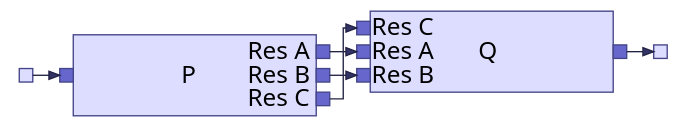
\includegraphics[scale=0.5]{img/swap_port_graph_alt.png}
  \caption{Process port graph involving \isa{Swap\ \isapars{Res\ A\ \isasymodot\ Res\ B}\ \isapars{Res\ C}}}
  \label{fig:swap_port_graph}
\end{figure}

For \isa{Duplicate} and \isa{Repeat} we use the same pattern: we build a port graph consisting of no node and one input port with two edges going from it to two output ports.
We call this pattern \isa{forkPortGraph}, parameterised by the single piece of data for all its open ports.
Its instance for duplicating a copyable atom \isa{data} is shown in Figure~\ref{fig:duplicate_port_graph}.

\begin{figure}[htbp]
  \centering
  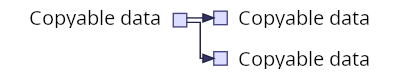
\includegraphics[scale=0.5]{img/duplicate_port_graph.png}
  \caption{Process port graph for \isa{Duplicate\ data}}
  \label{fig:duplicate_port_graph}
\end{figure}

For \isa{Erase} and \isa{Close} we use a very simple pattern: a single input port with no edges or output ports.
This represents closing off whatever output port this single input is composed with.
Its instance for erasing a copyable atom \isa{data} is shown in Figure~\ref{fig:erase_port_graph}.

\begin{figure}[htbp]
  \centering
  
\includegraphics[scale=0.5]{img/erase_port_graph.png}
  \caption{Process port graph for \isa{Erase\ data}}
  \label{fig:erase_port_graph}
\end{figure}

For \isa{Once} we use a pattern similar to \isa{Identity} but, because of how its input and output interact with \isa{parallel{\isacharunderscore}parts}, there is only one edge.
Moreover, the origin and destination of that edge carry different resources as data: the origin carries a \isa{Repeatable} resource while the destination carries the corresponding \isa{Executable} resource.
Note that this is the first port graph pattern we use in which the labels on origin and destination of an edge differ.
Its instance for a repeatable process from \isa{\isafv{x}} to \isa{\isafv{y}} is shown in Figure~\ref{fig:erase_port_graph}.

\begin{figure}[htbp]
  \centering
  
\includegraphics[scale=0.5]{img/once_port_graph.png}
  \caption{Process port graph for \isa{Once\ \isafv{x}\ \isafv{y}}}
  \label{fig:once_port_graph}
\end{figure}

For \isa{Forget} we build a port graph consisting of no node, a number of input ports and a single output port, and edges from every input to the sole output.
We use parallel parts of the input resource to label the input ports and the output \isa{Anything} resource to label the output port.
This represents any complex resource merging into a single \isa{Anything} resource, forgetting any details about it including that it may have consisted of multiple parts.
Note that in this port graph we also may have edges with origin and destination labelled differently.
Its instance for the resources \isa{Res\ A}, \isa{Res\ B} and \isa{Res\ C} is shown in Figure~\ref{fig:forget_port_graph}.

\begin{figure}[htbp]
  \centering
  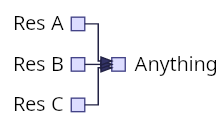
\includegraphics[scale=0.5]{img/forget_port_graph.png}
  \caption{Process port graph for \isa{Forget {Res\ A\ \isasymodot\ Res\ B}\ \isasymodot\ Res\ C}}
  \label{fig:forget_port_graph}
\end{figure}

This concludes the patterns we use to generate port graphs from process compositions.
Figure~\ref{fig:fourGears_port_graph} illustrates the port graph construction on a more complex process composition, the manufacturing of four iron gears per second defined in Section~\ref{sec:cases/factorio/gears}.
We next turn to the properties that our process port graphs satisfy.

\begin{figure}[htbp]
  \centering
  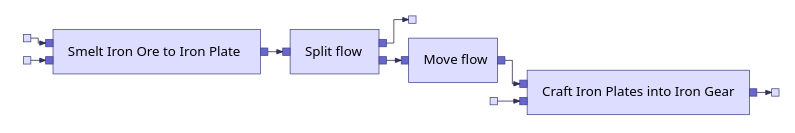
\includegraphics[scale=0.5]{img/fourGears_port_graph.png}
  \caption{Process port graph for manufacturing four iron gears per second (see Section~\ref{sec:cases/factorio/gears} for details of this process). We omit open port labels due to their size.}
  \label{fig:fourGears_port_graph}
\end{figure}

\subsection{Properties of Process Port Graphs}
\label{sec:port_graphs/process/prop}

Before we discuss specific properties, recall that our process port graph construction is not defined for processes that make use of non-deterministic or higher-order features.
\cbstart
To exclude such processes from consideration, we define the predicate \isa{pgDefined} (see Appendix~\ref{app:pgDefined} for its full definition).
We then assume that any process used in \isa{pgConstruct} satisfies this condition.
\cbend

We start our verification by proving that our construction, given a composition it is fully defined on, results in a well-formed port graph with flow.
Proving that each of the port graph patterns we use is well-formed and satisfies the flow requirements is quite simple, because having concrete port graphs simplifies much of the quantification in the locale assumptions.
The cases for parallel and sequential composition are simple, because we prove that both port graph juxtaposition and sequencing satisfy the \isa{port{\isacharunderscore}graph{\isacharunderscore}flow} locale just after defining them (Lemma~\ref{isa:port_graph_juxtapose} and Lemma~\ref{isa:port_graph_flow_seqPortGraphs}).
Therefore we now only need to prove that qualifying the child port graphs with distinct atoms (\isa{SeqL} and \isa{SeqR}, or \isa{ParL} and \isa{ParR}) indeed makes them disjoint, which is easily done.
As a result, we have the following theorem in Isabelle/HOL:
\begin{isalemma}[Process port graphs are well-formed]{isa:port_graph_flow_pgConstruct}
  \isacomm{lemma}\isamarkupfalse%
\ port{\isacharunderscore}graph{\isacharunderscore}flow{\isacharunderscore}pgConstruct{\isacharcolon}\isanewline
\ \ \isaOcomm{assumes}\ {\isachardoublequoteopen}pgDefined\ \isafv{x}{\isachardoublequoteclose}\isanewline
\ \ \ \ \ \ \isaOcomm{shows}\ {\isachardoublequoteopen}port{\isacharunderscore}graph{\isacharunderscore}flow\ {\isacharparenleft}pgConstruct\ \isafv{x}{\isacharparenright}{\isachardoublequoteclose}

\end{isalemma}

Then we show that the open ports of the constructed port graph correspond to parallel parts (given in Definition~\ref{isa:parallel_parts}) of the process composition's input and output resources:
\begin{isalemma}[Open ports correspond to input and output]{isa:pgConstruct_ports}
  \isacomm{lemma}\isamarkupfalse%
\ pgConstruct{\isacharunderscore}ports{\isacharcolon}\isanewline
\ \ \isaOcomm{assumes}\ {\isachardoublequoteopen}pgDefined\ \isafv{x}{\isachardoublequoteclose}\isanewline
\ \ \ \ \ \ \isaOcomm{shows}\ {\isachardoublequoteopen}set\ {\isacharparenleft}pg{\isacharunderscore}ports\ {\isacharparenleft}pgConstruct\ \isafv{x}{\isacharparenright}{\isacharparenright}\ {\isacharequal}\isanewline
\isaindent{\ \ \ \ \ \ \isaOcomm{shows}\ {\isachardoublequoteopen}}set\ {\isacharparenleft}parallelPorts\ {\isadigit{0}}\ In\ {\isacharparenleft}input\ \isafv{x}{\isacharparenright}\ {\isacharat}\ parallelPorts\ {\isadigit{0}}\ Out\ {\isacharparenleft}output\ \isafv{x}{\isacharparenright}{\isacharparenright}{\isachardoublequoteclose}

\end{isalemma}

Moreover, the nodes of the port graph also correspond to the primitive actions present in the process composition.
To prove this, we define the function \isa{namedPrimitives} that operates exactly as the function \isa{primitives} (see Section~\ref{sec:proc/type/primitive}) but also collects the path to each primitive action.
We show that the path is the node name, the action's label and metadata are the node label, and the action's input and output form the node ports:
\begin{isalemma}[Nodes correspond to primitive actions]{isa:pgConstruct_nodes}
  \isacomm{lemma}\ pgConstruct{\isacharunderscore}nodes{\isacharcolon}\isanewline
\ \ \isaOcomm{assumes}\ {\isachardoublequoteopen}pgDefined\ \isafv{x}{\isachardoublequoteclose}\isanewline
\ \ \ \ \ \ \isaOcomm{shows}\ pg{\isacharunderscore}nodes\ {\isacharparenleft}pgConstruct\ \isafv{x}{\isacharparenright}\ {\isacharequal}\isanewline
\isaindent{\ \ \ \ \ \ \isaOcomm{shows}\ }map\ {\isacharparenleft}{\isasymlambda}{\isacharparenleft}\isabv{n}{\isacharcomma}\ \isabv{ins}{\isacharcomma}\ \isabv{outs}{\isacharcomma}\ \isabv{l}{\isacharcomma}\ \isabv{m}{\isacharparenright}{\isachardot}\isanewline
\isaindent{\ \ \ \ \ \ \isaOcomm{shows}\ map\ {\isacharparenleft}{\isasymlambda}}Node\ \isabv{n}\ {\isacharparenleft}NodePrimitive\ \isabv{l\ m}{\isacharparenright}\ {\isacharparenleft}parallelPorts\ {\isadigit{0}}\ In\ \isabv{ins}\ {\isacharat}\isanewline
\isaindent{\ \ \ \ \ \ \isaOcomm{shows}\ map\ {\isacharparenleft}{\isasymlambda}Node\ \isabv{n}\ {\isacharparenleft}NodePrimitive\ \isabv{l\ m}{\isacharparenright}\ {\isacharparenleft}}parallelPorts\ {\isadigit{0}}\ Out\ \isabv{outs}{\isacharparenright}{\isacharparenright}\isanewline
\isaindent{\ \ \ \ \ \ \isaOcomm{shows}\ map\ }{\isacharparenleft}namedPrimitives\ \isafv{x}{\isacharparenright}{\isachardoublequoteclose}

\end{isalemma}

The remainder of the properties we highlight in this section concern situations where different process compositions yield equivalent port graphs.
These capture a deeper aspect of process compositions than the surface-level syntax: they say that two compositions, although syntactically different, represent the same structure of connections between actions.
In Section~\ref{sec:port_graphs/conc} we discuss future work taking further advantage of this aspect of the equivalence.

To start with, we can show that, up to equivalence of constructed port graphs, the identity process behaves as unit for both sequential and parallel composition:
\begin{isalemma}[Identity process is sequential unit]{isa:pgConstruct_seq_unit_pgEquiv}
  \isacomm{lemma}\ pgConstruct{\isacharunderscore}seq{\isacharunderscore}unit{\isacharunderscore}pgEquiv{\isacharcolon}\isanewline
\ \ \isaOcomm{assumes}\ {\isachardoublequoteopen}pgDefined\ \isafv{x}{\isachardoublequoteclose}\isanewline
\ \ \ \ \ \ \isaOcomm{shows}\ {\isachardoublequoteopen}pgConstruct\ {\isacharparenleft}Seq\ {\isacharparenleft}Identity\ {\isacharparenleft}input\ \isafv{x}{\isacharparenright}{\isacharparenright}\ \isafv{x}{\isacharparenright}\ {\isasymapprox}\ pgConstruct\ \isafv{x}{\isachardoublequoteclose}\isanewline
\ \ \ \ \ \ \ \ \ \ \isaOcomm{and}\ {\isachardoublequoteopen}pgConstruct\ {\isacharparenleft}Seq\ \isafv{x}\ {\isacharparenleft}Identity\ {\isacharparenleft}output\ \isafv{x}{\isacharparenright}{\isacharparenright}{\isacharparenright}\ {\isasymapprox}\ pgConstruct\ \isafv{x}{\isachardoublequoteclose}

\end{isalemma}
\pagebreak
\begin{isalemma}[Identity process is parallel unit]{isa:pgConstruct_par_unit_pgEquiv}
  \isacomm{lemma}\ pgConstruct{\isacharunderscore}par{\isacharunderscore}unit{\isacharunderscore}pgEquiv{\isacharcolon}\isanewline
\ \ \isaOcomm{assumes}\ {\isachardoublequoteopen}pgDefined\ \isafv{x}{\isachardoublequoteclose}\isanewline
\ \ \ \ \ \ \isaOcomm{shows}\ {\isachardoublequoteopen}pgConstruct\ {\isacharparenleft}Par\ {\isacharparenleft}Identity\ Empty{\isacharparenright}\ \isafv{x}{\isacharparenright}\ {\isasymapprox}\ pgConstruct\ \isafv{x}{\isachardoublequoteclose}\isanewline
\ \ \ \ \ \ \ \ \ \ \isaOcomm{and}\ {\isachardoublequoteopen}pgConstruct\ {\isacharparenleft}Par\ \isafv{x}\ {\isacharparenleft}Identity\ Empty{\isacharparenright}{\isacharparenright}\ {\isasymapprox}\ pgConstruct\ \isafv{x}{\isachardoublequoteclose}

\end{isalemma}

We can also take the theorems about when port graph sequencing and juxtaposition are associative and show that the process port graphs satisfy their assumptions.
This is because qualifying port graphs with distinct name atoms makes them disjoint while being equivalent to the original.
As a result, we get the following two theorems:
\begin{isalemma}[Parallel and sequential composition are associative]{isa:pgConstruct_assoc}
  \isacomm{lemma}\isanewline
\ \ \isaOcomm{assumes}\ {\isachardoublequoteopen}pgDefined\ \isafv{x}{\isachardoublequoteclose}\ \isaOcomm{and}\ {\isachardoublequoteopen}pgDefined\ \isafv{y}{\isachardoublequoteclose}\ \isaOcomm{and}\ {\isachardoublequoteopen}pgDefined\ \isafv{z}{\isachardoublequoteclose}\isanewline
\ \ \ \ \ \ \isaOcomm{shows}\ pgConstruct{\isacharunderscore}Par{\isacharunderscore}assoc{\isacharcolon}\isanewline
\isaindent{\ \ \ \ \ \ \isaOcomm{shows}\ }{\isachardoublequoteopen}pgConstruct\ {\isacharparenleft}Par\ {\isacharparenleft}Par\ \isafv{x\ y}{\isacharparenright}\ \isafv{z}{\isacharparenright}\ {\isasymapprox}\ pgConstruct\ {\isacharparenleft}Par\ \isafv{x}\ {\isacharparenleft}Par\ \isafv{y\ z}{\isacharparenright}{\isacharparenright}{\isachardoublequoteclose}\isanewline
\ \ \ \ \ \ \ \ \ \ \isaOcomm{and}\ pgConstruct{\isacharunderscore}Seq{\isacharunderscore}assoc{\isacharcolon}\isanewline
\isaindent{\ \ \ \ \ \ \ \ \ \ \isaOcomm{and}\ }{\isachardoublequoteopen}pgConstruct\ {\isacharparenleft}Seq\ {\isacharparenleft}Seq\ \isafv{x\ y}{\isacharparenright}\ \isafv{z}{\isacharparenright}\ {\isasymapprox}\ pgConstruct\ {\isacharparenleft}Seq\ \isafv{x}\ {\isacharparenleft}Seq\ \isafv{y\ z}{\isacharparenright}{\isacharparenright}{\isachardoublequoteclose}

\end{isalemma}

And we can show that the \isa{Duplicate} action forms a monoid in this way with the \isa{Erase} action as unit: erasing either result of duplication is as if we did nothing, and nesting duplications is associative.
Because the corresponding port graphs have no nodes that would require renaming, the relations can be shown as \emph{equalities} of port graphs instead of just equivalences.
All three statements are as follows:
\begin{isalemma}[\isa{Duplicate} and \isa{Erase} form a monoid]{isa:pgConstruct_duplicate_erase}
  \isacomm{lemma}\isamarkupfalse%
\isanewline
\ \ \isaOcomm{shows}\ pgConstruct{\isacharunderscore}duplicate{\isacharunderscore}eraseL{\isacharcolon}\isanewline
\ \ \ \ pgConstruct\ {\isacharparenleft}Seq\ {\isacharparenleft}Duplicate\ \isafv{x}{\isacharparenright}\ {\isacharparenleft}Par\ {\isacharparenleft}Erase\ \isafv{x}{\isacharparenright}\ {\isacharparenleft}Identity\ {\isacharparenleft}Copyable\ \isafv{x}{\isacharparenright}{\isacharparenright}{\isacharparenright}{\isacharparenright}\ {\isacharequal}\isanewline
\ \ \ \ pgConstruct\ {\isacharparenleft}Identity\ {\isacharparenleft}Copyable\ \isafv{x}{\isacharparenright}{\isacharparenright}{\isachardoublequoteclose}\isanewline
\ \ \ \ \ \ \isaOcomm{and}\ pgConstruct{\isacharunderscore}duplicate{\isacharunderscore}eraseR{\isacharcolon}\isanewline
\ \ \ \ pgConstruct\ {\isacharparenleft}Seq\ {\isacharparenleft}Duplicate\ \isafv{x}{\isacharparenright}\ {\isacharparenleft}Par\ {\isacharparenleft}Identity\ {\isacharparenleft}Copyable\ \isafv{x}{\isacharparenright}{\isacharparenright}\ {\isacharparenleft}Erase\ \isafv{x}{\isacharparenright}{\isacharparenright}{\isacharparenright}\ {\isacharequal}\isanewline
\ \ \ \ pgConstruct\ {\isacharparenleft}Identity\ {\isacharparenleft}Copyable\ \isafv{x}{\isacharparenright}{\isacharparenright}{\isachardoublequoteclose}\isanewline
\ \ \ \ \ \ \isaOcomm{and}\ pgConstruct{\isacharunderscore}duplicate{\isacharunderscore}assoc{\isacharcolon}\isanewline
\ \ \ \ pgConstruct\ {\isacharparenleft}Seq\ {\isacharparenleft}Duplicate\ \isafv{x}{\isacharparenright}\ {\isacharparenleft}Par\ {\isacharparenleft}Identity\ {\isacharparenleft}Copyable\ \isafv{x}{\isacharparenright}{\isacharparenright}\ {\isacharparenleft}Duplicate\ \isafv{x}{\isacharparenright}{\isacharparenright}{\isacharparenright}\ {\isacharequal}\isanewline
\ \ \ \ pgConstruct\ {\isacharparenleft}Seq\ {\isacharparenleft}Duplicate\ \isafv{x}{\isacharparenright}\ {\isacharparenleft}Par\ {\isacharparenleft}Duplicate\ \isafv{x}{\isacharparenright}\ {\isacharparenleft}Identity\ {\isacharparenleft}Copyable\ \isafv{x}{\isacharparenright}{\isacharparenright}{\isacharparenright}{\isacharparenright}{\isachardoublequoteclose}

\end{isalemma}

Increasing the statement complexity, we can prove {\cbstart}that any process that composes like an identity action produces a port graph equivalent to it.
More precisely, by composing like an identity action we mean that
\begin{enumerate*}[label=(\roman*)]
  \item sequential composition of the candidate process with itself is valid, and
  \item for any other process whose sequential composition with the candidate is valid the result produces a port graph equivalent to that other process.
\end{enumerate*}
This yields two theorems, Lemma~\ref{isa:pgConstruct_ide_input} and Lemma~\ref{isa:pgConstruct_ide_output}, which differ in the ordering of the sequential composition and thus in the identity action using the input or output resource.
\cbend

\begin{isalemma}[Left unit of \isa{Seq} is equivalent to an identity on input]{isa:pgConstruct_ide_input}
  \isacomm{lemma}\isamarkupfalse%
\ pgConstruct{\isacharunderscore}ide{\isacharunderscore}input{\isacharcolon}\isanewline
\ \ \isaOcomm{assumes}\ {\isachardoublequoteopen}pgDefined\ \isafv{x}{\isachardoublequoteclose}\isanewline
\ \ \ \ \ \ \ \ \ \ \isaOcomm{and}\ {\isachardoublequoteopen}valid\ {\isacharparenleft}Seq\ \isafv{x\ x}{\isacharparenright}{\isachardoublequoteclose}\isanewline
\ \ \ \ \ \ \ \ \ \ \isaOcomm{and}\ {\isachardoublequoteopen}{\isasymAnd}\isabv{f}{\isachardot}\ {\isasymlbrakk}pgDefined\ \isabv{f}{\isacharsemicolon}\ valid\ {\isacharparenleft}Seq\ \isabv{f}\ \isafv{x}{\isacharparenright}{\isasymrbrakk}\isanewline
\isaindent{\ \ \ \ \ \ \ \ \ \ \isaOcomm{and}\ {\isachardoublequoteopen}{\isasymAnd}\isabv{f}{\isachardot}\ }{\isasymLongrightarrow}\ pgConstruct\ {\isacharparenleft}Seq\ \isabv{f}\ \isafv{x}{\isacharparenright}\ {\isasymapprox}\ pgConstruct\ \isabv{f}{\isachardoublequoteclose}\isanewline
\ \ \ \ \ \ \isaOcomm{shows}\ {\isachardoublequoteopen}pgConstruct\ \isafv{x}\ {\isasymapprox}\ pgConstruct\ {\isacharparenleft}Identity\ {\isacharparenleft}input\ \isafv{x}{\isacharparenright}{\isacharparenright}{\isachardoublequoteclose}

\end{isalemma}
\begin{isalemma}[Right unit of \isa{Seq} is equivalent to an identity on output]{isa:pgConstruct_ide_output}
  \isacomm{lemma}\isamarkupfalse%
\ pgConstruct{\isacharunderscore}ide{\isacharunderscore}output{\isacharcolon}\isanewline
\ \ \isaOcomm{assumes}\ {\isachardoublequoteopen}pgDefined\ \isafv{x}{\isachardoublequoteclose}\isanewline
\ \ \ \ \ \ \ \ \ \ \isaOcomm{and}\ {\isachardoublequoteopen}valid\ {\isacharparenleft}Seq\ \isafv{x\ x}{\isacharparenright}{\isachardoublequoteclose}\isanewline
\ \ \ \ \ \ \ \ \ \ \isaOcomm{and}\ {\isachardoublequoteopen}{\isasymAnd}\isabv{f}{\isachardot}\ {\isasymlbrakk}pgDefined\ \isabv{f}{\isacharsemicolon}\ valid\ {\isacharparenleft}Seq\ \isafv{x}\ \isabv{f}{\isacharparenright}{\isasymrbrakk}\isanewline
\isaindent{\ \ \ \ \ \ \ \ \ \ \isaOcomm{and}\ {\isachardoublequoteopen}{\isasymAnd}\isabv{f}{\isachardot}\ }{\isasymLongrightarrow}\ pgConstruct\ {\isacharparenleft}Seq\ \isafv{x}\ \isabv{f}{\isacharparenright}\ {\isasymapprox}\ pgConstruct\ \isabv{f}{\isachardoublequoteclose}\isanewline
\ \ \ \ \ \ \isaOcomm{shows}\ {\isachardoublequoteopen}pgConstruct\ \isafv{x}\ {\isasymapprox}\ pgConstruct\ {\isacharparenleft}Identity\ {\isacharparenleft}output\ \isafv{x}{\isacharparenright}{\isacharparenright}{\isachardoublequoteclose}

\end{isalemma}

In the following two sections we turn to two statements about processes that this new graphical perspective allows us to prove.
One describes when parallel and sequential composition of processes can pass through each other without affecting the connections between actions.
The other characterises the range of connections that can occur in valid process compositions, serving as a graphical counterpart to our demonstration of linearity in Chapter~\ref{ch:linearity}.

\section{Process Interchange}
\label{sec:port_graphs/interchange}

In general, parallel and sequential composition of processes do not distribute over each other.
(For a more thorough discussion of behaviour one expects from concurrent programs and process calculi, see Hoare and van~Staden~\cite{hoare_staden-2014}.)
In our notation, this means we would expect \isa{Seq\ \isapars{Par\ \isafv{R\ S}}\ \isapars{Par\ \isafv{T\ U}}} to have more constrained behaviour than \isa{Par\ \isapars{Seq\ \isafv{R\ T}}\ \isapars{Seq\ \isafv{S\ U}}} (when they are both valid compositions).
This is because, in a direct reading, the latter form allows for more interleaving of the processes: the former stipulates that we do \isa{\isafv{R}} and\ \isa{\isafv{S}} before \isa{\isafv{T}} and\ \isa{\isafv{U}}, while the latter allows us to do \isa{\isafv{T}} before \isa{\isafv{S}} as long as it follows \isa{\isafv{R}}.
In practice, this may for instance be the case if \isa{\isafv{U}} depends on \isa{\isafv{R}} in order to execute.

However, for both forms to be valid in our framework we must have \isa{output\ \isafv{R}\ \isacharequal\ input\ \isafv{T}} and \isa{output\ \isafv{S}\ \isacharequal\ input\ \isafv{U}}.
Note that this means there is no resource passing from \isa{\isafv{R}} to \isa{\isafv{U}} and from \isa{\isafv{S}} to \isa{\isafv{T}}.
And, because resources in our framework model dependency between actions, we would expect to be able to do \isa{\isafv{T}} without first doing \isa{\isafv{S}}.
Because through resources in our framework we have this extra information about the dependency between actions, we would like to equate the two forms when both are valid.

We cannot equate the two forms in themselves, because they are different compositions of processes.
But, because our claim about their close relation is based in connections, we can relate them through the port graphs they generate.
A simple indication of this is that, when \cbar{both} compositions are valid, our implementation of process diagrams (see Section~\ref{sec:proc/diag}) draws the same diagram for both, shown in Figure~\ref{fig:interchange-diag}.

\begin{figure}[hbtp]
  \centering
  \includesvg[scale=1]{img-gen/interchange.svg}
  \caption{Common process diagram for the compositions \isa{Seq\ \isapars{Par\ \isafv{R\ S}}\ \isapars{Par\ \isafv{T\ U}}} and \isa{Par\ \isapars{Seq\ \isafv{R\ T}}\ \isapars{Seq\ \isafv{S\ U}}}}
  \label{fig:interchange-diag}
\end{figure}

With our process port graphs, we can make this relation fully formal: for any four processes, if both the composition forms are valid then the port graphs resulting from them are equivalent.
Note that validity of one subsumes validity of the other, so we need only assume one is valid.
That is, in Isabelle/HOL:
\begin{isalemma}[Interchange of process port graphs]{isa:pgConstruct_interchange}
  \isacomm{lemma}\ pgConstruct{\isacharunderscore}interchange{\isacharcolon}\isanewline
\ \ \isaOcomm{assumes}\ {\isachardoublequoteopen}pgDefined\ \isafv{r}{\isachardoublequoteclose}\ \isaOcomm{and}\ {\isachardoublequoteopen}pgDefined\ \isafv{t}{\isachardoublequoteclose}\ \isaOcomm{and}\ {\isachardoublequoteopen}pgDefined\ \isafv{s}{\isachardoublequoteclose}\ \isaOcomm{and}\ {\isachardoublequoteopen}pgDefined\ \isafv{u}{\isachardoublequoteclose}\isanewline
\ \ \ \ \ \ \ \ \ \ \isaOcomm{and}\ {\isachardoublequoteopen}valid\ {\isacharparenleft}Par\ {\isacharparenleft}Seq\ \isafv{r\ t}{\isacharparenright}\ {\isacharparenleft}Seq\ \isafv{s\ u}{\isacharparenright}{\isacharparenright}{\isachardoublequoteclose}\isanewline
\ \ \ \ \ \ \isaOcomm{shows}\ {\isachardoublequoteopen}pgConstruct\ {\isacharparenleft}Seq\ {\isacharparenleft}Par\ \isafv{r\ s}{\isacharparenright}\ {\isacharparenleft}Par\ \isafv{t\ u}{\isacharparenright}{\isacharparenright}\ {\isasymapprox}\isanewline
\isaindent{\ \ \ \ \ \ \isaOcomm{shows}\ {\isachardoublequoteopen}}pgConstruct\ {\isacharparenleft}Par\ {\isacharparenleft}Seq\ \isafv{r\ t}{\isacharparenright}\ {\isacharparenleft}Seq\ \isafv{s\ u}{\isacharparenright}{\isacharparenright}{\isachardoublequoteclose}

\end{isalemma}

We prove this fact first as a general theorem about port graphs and then show that process port graphs satisfy its assumptions.
In that, we again use the fact that port graph qualification done as part of the construction makes the child port graphs disjoint while keeping them equivalent to the originals, and that process port graphs only use the input and output sides for ports.
Beyond all the parameters being well-formed port graphs with flow that are disjoint from each other, there are two interesting assumptions we need to satisfy.
They require that the number of output ports of \isa{pgConstruct\ \isafv{r}} must be equal to the number of input ports of \isa{pgConstruct\ \isafv{t}}, and the same for \isa{\isafv{s}} and \isa{\isafv{u}} respectively.
We prove these for process port graphs from the validity assumption and the fact that open ports of process port graphs correspond to the inputs and outputs of the relevant process.

As a result, while the two compositions are syntactically distinct and in the general context of concurrent process modelling we would not expect them to be the same, we can use the extra information expressed by resources in our framework and our connection to port graphs to prove when they result in the same connections between actions.
Figure~\ref{fig:interchange_port_graph} visualises the port graph that results from both forms, which, as expected, matches the unformalised process diagram in Figure~\ref{fig:interchange-diag}.

\begin{figure}[hbtp]
  \centering
  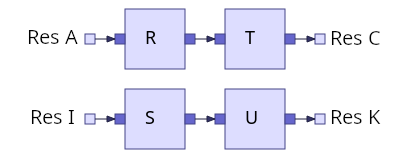
\includegraphics[scale=0.5]{img/interchange_port_graph.png}
  \caption{Port graph for both forms of nested parallel and sequential composition}
  \label{fig:interchange_port_graph}
\end{figure}

\section{Graphical Linearity}
\label{sec:port_graphs/linearity}

Our work in Chapter~\ref{ch:linearity} demonstrates process correctness, more specifically their linearity, by appealing to linear logic.
We transform all process compositions into deductions in linear logic while preserving their structure and then prove that for valid compositions the resulting deduction follows the rules of linear logic.

However, that demonstration does not say what linearity means directly in terms of the resources and processes, just that adherence to the rules of linear logic demonstrates it.
In this section we use our port graph construction to split all occurrences of resources in the process (represented by places of the constructed port graph) into five categories based on how they connect to other occurrences.
This characterises all the ways resources are manipulated in the process and allows us to then argue that they are being manipulated correctly by addressing each category.
\cbar{We first present the formal statement, followed by discussion of the cases it identifies.}

\pagebreak
\begin{isalemma}[Graphical linearity of process port graphs]{isa:pgConstruct_linearity}
  \isacomm{lemma}\ pgConstruct{\isacharunderscore}linearity{\isacharcolon}\isanewline
\ \ \isaOcomm{assumes}\ {\isachardoublequoteopen}pgDefined\ \isafv{x}{\isachardoublequoteclose}\ \isaOcomm{and}\ {\isachardoublequoteopen}valid\ \isafv{x}{\isachardoublequoteclose}\isanewline
\ \ \widthtoL{\isaOcomm{and}}{\isaOcomm{assumes}}\ {\isachardoublequoteopen}\isafv{p}\ {\isasymin}\ set\ {\isacharparenleft}pgraphPlaces\ {\isacharparenleft}pgConstruct\ \isafv{x}{\isacharparenright}{\isacharparenright}{\isachardoublequoteclose}\isanewline
\ \ \widthtoL{\isaOcomm{obtains}}{\isaOcomm{assumes}}\isanewline
\ \ \isaindent{\isacharbar\ }{\isacharparenleft}Linear{\isacharparenright}\isanewline
\ \ \isaindent{\isaOcomm{assumes}\ }{\isachardoublequoteopen}{\isasymnot}{\isacharparenleft}{\isasymexists}\isabv{a}{\isachardot}\ port{\isachardot}label\ {\isacharparenleft}place{\isacharunderscore}port\ \isafv{p}{\isacharparenright}\ {\isacharequal}\ Copyable\ \isabv{a}{\isacharparenright}{\isachardoublequoteclose}\isanewline
\ \ \widthtoL{\isaOcomm{and}}{\isaOcomm{assumes}}\ {\isachardoublequoteopen}{\isasymnot}{\isacharparenleft}{\isasymexists}\isabv{a\ b}{\isachardot}\ port{\isachardot}label\ {\isacharparenleft}place{\isacharunderscore}port\ \isafv{p}{\isacharparenright}\ {\isacharequal}\ Repeatable\ \isabv{a\ b}{\isacharparenright}{\isachardoublequoteclose}\isanewline
\ \ \widthtoL{\isaOcomm{and}}{\isaOcomm{assumes}}\ {\isachardoublequoteopen}port{\isachardot}label\ {\isacharparenleft}place{\isacharunderscore}port\ \isafv{p}{\isacharparenright}\ {\isasymnoteq}\ Anything{\isachardoublequoteclose}\isanewline
\ \ \widthtoL{\isaOcomm{and}}{\isaOcomm{assumes}}\ {\isachardoublequoteopen}{\isasymexists}{\isacharbang}\isabv{e}\ {\isasymin}\ set\ {\isacharparenleft}pg{\isacharunderscore}edges\ {\isacharparenleft}pgConstruct\ \isafv{x}{\isacharparenright}{\isacharparenright}{\isachardot}\ edge{\isacharunderscore}from\ \isabv{e}\ {\isacharequal}\ \isafv{p}\ {\isasymor}\ edge{\isacharunderscore}to\ \isabv{e}\ {\isacharequal}\ \isafv{p}{\isachardoublequoteclose}\isanewline
\ \ {\isacharbar}\ {\isacharparenleft}NonLinear{\isacharunderscore}Origin{\isacharparenright}\isanewline
\ \ \isaindent{\isaOcomm{assumes}\ }{\isachardoublequoteopen}{\isacharparenleft}{\isasymexists}\isabv{a}{\isachardot}\ port{\isachardot}label\ {\isacharparenleft}place{\isacharunderscore}port\ \isafv{p}{\isacharparenright}\ {\isacharequal}\ Copyable\ \isabv{a}{\isacharparenright}\ {\isasymor}\isanewline
\ \ \isaindent{\isaOcomm{assumes}\ }{\isacharparenleft}{\isasymexists}\isabv{a\ b}{\isachardot}\ port{\isachardot}label\ {\isacharparenleft}place{\isacharunderscore}port\ \isafv{p}{\isacharparenright}\ {\isacharequal}\ Repeatable\ \isabv{a\ b}{\isacharparenright}{\isachardoublequoteclose}\isanewline
\ \ \widthtoL{\isaOcomm{and}}{\isaOcomm{assumes}}\ {\isachardoublequoteopen}{\isasymnot}{\isacharparenleft}{\isasymexists}\isabv{e}\ {\isasymin}\ set\ {\isacharparenleft}pg{\isacharunderscore}edges\ {\isacharparenleft}pgConstruct\ \isafv{x}{\isacharparenright}{\isacharparenright}{\isachardot}\ edge{\isacharunderscore}to\ \isabv{e}\ {\isacharequal}\ \isafv{p}{\isacharparenright}{\isachardoublequoteclose}\isanewline
\ \ {\isacharbar}\ {\isacharparenleft}NonLinear{\isacharunderscore}Destin{\isacharparenright}\isanewline
\ \ \isaindent{\isaOcomm{assumes}\ }{\isachardoublequoteopen}{\isacharparenleft}{\isasymexists}\isabv{a}{\isachardot}\ port{\isachardot}label\ {\isacharparenleft}place{\isacharunderscore}port\ \isafv{p}{\isacharparenright}\ {\isacharequal}\ Copyable\ \isabv{a}{\isacharparenright}\ {\isasymor}\isanewline
\ \ \isaindent{\isaOcomm{assumes}\ }{\isacharparenleft}{\isasymexists}\isabv{a\ b}{\isachardot}\ port{\isachardot}label\ {\isacharparenleft}place{\isacharunderscore}port\ \isafv{p}{\isacharparenright}\ {\isacharequal}\ Repeatable\ \isabv{a\ b}{\isacharparenright}{\isachardoublequoteclose}\isanewline
\ \ \widthtoL{\isaOcomm{and}}{\isaOcomm{assumes}}\ {\isachardoublequoteopen}{\isasymnot}{\isacharparenleft}{\isasymexists}\isabv{e}\ {\isasymin}\ set\ {\isacharparenleft}pg{\isacharunderscore}edges\ {\isacharparenleft}pgConstruct\ \isafv{x}{\isacharparenright}{\isacharparenright}{\isachardot}\ edge{\isacharunderscore}from\ \isabv{e}\ {\isacharequal}\ \isafv{p}{\isacharparenright}{\isachardoublequoteclose}\isanewline
\ \ \widthtoL{\isaOcomm{and}}{\isaOcomm{assumes}}\ {\isachardoublequoteopen}{\isasymexists}{\isacharbang}\isabv{e}\ {\isasymin}\ set\ {\isacharparenleft}pg{\isacharunderscore}edges\ {\isacharparenleft}pgConstruct\ \isafv{x}{\isacharparenright}{\isacharparenright}{\isachardot}\ edge{\isacharunderscore}to\ \isabv{e}\ {\isacharequal}\ \isafv{p}{\isachardoublequoteclose}\isanewline
\ \ {\isacharbar}\ {\isacharparenleft}Anything{\isacharunderscore}Origin{\isacharparenright}\isanewline
\ \ \isaindent{\isaOcomm{assumes}\ }{\isachardoublequoteopen}port{\isachardot}label\ {\isacharparenleft}place{\isacharunderscore}port\ \isafv{p}{\isacharparenright}\ {\isacharequal}\ Anything{\isachardoublequoteclose}\isanewline
\ \ \widthtoL{\isaOcomm{and}}{\isaOcomm{assumes}}\ {\isachardoublequoteopen}{\isasymexists}{\isacharbang}\isabv{e}\ {\isasymin}\ set\ {\isacharparenleft}pg{\isacharunderscore}edges\ {\isacharparenleft}pgConstruct\ \isafv{x}{\isacharparenright}{\isacharparenright}{\isachardot}\ edge{\isacharunderscore}from\ \isabv{e}\ {\isacharequal}\ \isafv{p}{\isachardoublequoteclose}\isanewline
\ \ \widthtoL{\isaOcomm{and}}{\isaOcomm{assumes}}\ {\isachardoublequoteopen}{\isasymnot}{\isacharparenleft}{\isasymexists}\isabv{e}\ {\isasymin}\ set\ {\isacharparenleft}pg{\isacharunderscore}edges\ {\isacharparenleft}pgConstruct\ \isafv{x}{\isacharparenright}{\isacharparenright}{\isachardot}\ edge{\isacharunderscore}to\ \isabv{e}\ {\isacharequal}\ \isafv{p}{\isacharparenright}{\isachardoublequoteclose}\isanewline
\ \ {\isacharbar}\ {\isacharparenleft}Anything{\isacharunderscore}Destin{\isacharparenright}\isanewline
\ \ \isaindent{\isaOcomm{assumes}\ }{\isachardoublequoteopen}port{\isachardot}label\ {\isacharparenleft}place{\isacharunderscore}port\ \isafv{p}{\isacharparenright}\ {\isacharequal}\ Anything{\isachardoublequoteclose}\isanewline
\ \ \widthtoL{\isaOcomm{and}}{\isaOcomm{assumes}}\ {\isachardoublequoteopen}{\isasymnot}{\isacharparenleft}{\isasymexists}\isabv{e}\ {\isasymin}\ set\ {\isacharparenleft}pg{\isacharunderscore}edges\ {\isacharparenleft}pgConstruct\ \isafv{x}{\isacharparenright}{\isacharparenright}{\isachardot}\ edge{\isacharunderscore}from\ \isabv{e}\ {\isacharequal}\ \isafv{p}{\isacharparenright}{\isachardoublequoteclose}

\end{isalemma}

\cbstart
As with other properties of process port graphs up to this point, we start by assuming that the process \isa{\isafv{x}} in question has no non-deterministic or higher-order features.
Additionally, we assume that it is valid.
While that is not always needed for the resulting port graph to have certain properties (such as Lemma~\ref{isa:pgConstruct_ports}), it is vital in this case.
Then we fix a place \isa{\isafv{p}} in the port graph constructed from \isa{\isafv{x}} and prove that each such place falls into one of five cases:
\cbend
\begin{itemize}
  \item It is labelled with a linear resource and there is a unique edge incident on it, or
  \item It carries a copyable or repeatable resource (\isa{Copyable} or \isa{Repeatable}) and:
    \begin{itemize}
      \item there is no edge coming into it but an arbitrary number of edges coming from it, or
      \item there is no edge coming from it but there is a unique edge coming into it; or
    \end{itemize}
  \item It carries the \isa{Anything} resource and:
    \begin{itemize}
      \item there is a unique edge coming from it but no edge coming into it, or
      \item there is a no edge coming from it but an arbitrary number of edges coming into it.
    \end{itemize}
\end{itemize}

The proof of this theorem consists of six major sub-lemmas totalling around 2500 lines of Isabelle script.
Each proceeds by induction on the process composition structure, and case analysis covering the possible resource labels and incident edges.
In each case we simplify the port graph construction and arrive either at a pattern fitting one of the above five cases or a contradiction, meaning that incompatible pattern cannot arise by constructing a port graph from a valid process composition.

One crucial fact used in this proof is that all edges in the port graph construction have the same resource label on their origin and their destination, except for those turning a \isa{Repeatable} resource into an \isa{Executable} resource or any resource into the \isa{Anything} resource.
This allows us to prove that our goal property is preserved through sequencing of port graphs.

Let us now discuss in more detail the five cases into which this theorem splits connections in process port graphs, along with what they mean for the resources involved.

The first case is the most important: every linear resource (i.e.\ not copyable, repeatable or \isa{Anything}) is moved from exactly one origin to exactly one destination.
As a result, no linear resource is left where it is produced or used to satisfy multiple requirements, and every action requiring a linear resource has a unique source for it.

The remaining cases characterise the allowed exceptions to the first case.
The second and third cases say that copyable and repeatable resources can link to any number of destinations but must still have a unique origin.
That is, they can be copied and erased, but not merged.

The fourth and fifth cases say that the \isa{Anything} resource can be made by merging any number of other resources but after formation must be treated linearly.
This represents the idea of \isa{Anything} as grouping together arbitrary resources and treating them as one homogeneous object, which is then still a resource and must be treated as such.

With reference to our use of linear logic for similar purposes in Chapter~\ref{ch:linearity}, the first case corresponds to the base way how linear logic manipulates propositions, while the second and third cases correspond to the extra allowances for the \isa{\isacharbang} modality and the fourth and fifth cases correspond to the extra allowances of the \isa{\isasymbottom} proposition.
However, here we are explicitly using the language of connections between nodes which represent primitive actions.

Note that, because our present port graph construction does not cover all process compositions, this does not supersede the demonstration through linear logic.
Nevertheless, it offers a valuable perspective on the same high-level issue of process composition correctness and shows that our graphical approach detailed in this chapter can be fruitfully applied to verifying process models.

\section{Port Graph Transition System}
\label{sec:port_graphs/trans}

So far this chapter, we have been using port graphs to represent the structure of a process composition in a way inspired by the process diagrams of Section~\ref{sec:proc/diag}.
We can, however, form an additional relationship between port graphs and processes: behaviour, expressed as a transition system.
In this section we describe a transition system on port graphs, which in turn induces a transition system on process compositions through the port graphs constructed from them.
That in turn allows us to better formalise the meaning of different process compositions.

The intuition behind the port graph transition system relies on viewing nodes as actions and edges as dependencies between them, just as we do with process port graphs.
To make a transition, we find a node that has no incoming edge from another node.
This represents its lack of dependency on any other node.
Then we remove that node and all its adjacent edges from the port graph, which represents performing that action and distributing its results.
In the absence of dependency loops, this will either result in another transition candidate or a port graph with no more nodes.

In our mechanisation of this idea, we start by defining the \emph{node flow}.
This relation orders nodes based on the edges going between them, placing one node before another node if there is an edge from a port of the former to a port of the latter.
In Isabelle/HOL we define this as an inductive relation:
\begin{isadef}[Node flow]{isa:node_flow}
  \isacomm{inductive}\ node{\isacharunderscore}flow\ {\isacharcolon}{\isacharcolon}\ {\isachardoublequoteopen}{\isacharparenleft}\isatv{s}{\isacharcomma}\ \isatv{a}{\isacharcomma}\ \isatv{p}{\isacharcomma}\ \isatv{l}{\isacharparenright}\ port{\isacharunderscore}graph\isanewline
\isaindent{\isacomm{inductive}\ node{\isacharunderscore}flow\ }{\isasymRightarrow}\ {\isacharparenleft}\isatv{s}{\isacharcomma}\ \isatv{a}{\isacharcomma}\ \isatv{p}{\isacharcomma}\ \isatv{l}{\isacharparenright}\ node\ {\isasymRightarrow}\ {\isacharparenleft}\isatv{s}{\isacharcomma}\ \isatv{a}{\isacharcomma}\ \isatv{p}{\isacharcomma}\ \isatv{l}{\isacharparenright}\ node\ {\isasymRightarrow}\ bool{\isachardoublequoteclose}\isanewline
\ \ \isaOcomm{where}\isanewline
\ \ \ \ {\isachardoublequoteopen}{\isasymlbrakk}\isabv{x}\ {\isasymin}\ set\ {\isacharparenleft}pg{\isacharunderscore}nodes\ \isabv{G}{\isacharparenright}{\isacharsemicolon}\ \isabv{y}\ {\isasymin}\ set\ {\isacharparenleft}pg{\isacharunderscore}nodes\ \isabv{G}{\isacharparenright}{\isacharsemicolon}\ \isabv{e}\ {\isasymin}\ set\ {\isacharparenleft}pg{\isacharunderscore}edges\ \isabv{G}{\isacharparenright}{\isacharsemicolon}\isanewline
\isaindent{\ \ \ \ {\isachardoublequoteopen}{\isasymlbrakk}}edge{\isacharunderscore}from\ \isabv{e}\ {\isasymin}\ set\ {\isacharparenleft}nodePlaces\ \isabv{x}{\isacharparenright}{\isacharsemicolon}\ edge{\isacharunderscore}to\ \isabv{e}\ {\isasymin}\ set\ {\isacharparenleft}nodePlaces\ \isabv{y}{\isacharparenright}{\isasymrbrakk}\isanewline
\isaindent{\ \ \ \ {\isachardoublequoteopen}}{\isasymLongrightarrow}\ \isafv{node{\isacharunderscore}flow}\ \isabv{G\ x\ y}{\isachardoublequoteclose}

\end{isadef}

We can then define the concept of an \emph{enabled} node of a port graph, which is a node with no incoming edge that originates from another node:
\begin{isadef}[Enabled node]{isa:nodeEnabled}
  \isacomm{definition}\ nodeEnabled\ {\isacharcolon}{\isacharcolon}\ {\isachardoublequoteopen}{\isacharparenleft}\isatv{s}{\isacharcomma}\ \isatv{a}{\isacharcomma}\ \isatv{p}{\isacharcomma}\ \isatv{l}{\isacharparenright}\ port{\isacharunderscore}graph\ {\isasymRightarrow}\ {\isacharparenleft}\isatv{s}{\isacharcomma}\ \isatv{a}{\isacharcomma}\ \isatv{p}{\isacharcomma}\ \isatv{l}{\isacharparenright}\ node\ {\isasymRightarrow}\ bool{\isachardoublequoteclose}\isanewline
\ \ \isaOcomm{where}\ {\isachardoublequoteopen}\isafv{nodeEnabled}\ \isabv{G\ n}\ {\isasymequiv}\isanewline
\ \ \ \ \isabv{n}\ {\isasymin}\ set\ {\isacharparenleft}pg{\isacharunderscore}nodes\ \isabv{G}{\isacharparenright}\ {\isasymand}\isanewline
\ \ \ \ {\isacharparenleft}{\isasymforall}\isabv{e}{\isachardot}\ \isabv{e}\ {\isasymin}\ set\ {\isacharparenleft}pg{\isacharunderscore}edges\ \isabv{G}{\isacharparenright}\ {\isasymand}\ place{\isacharunderscore}ground\ {\isacharparenleft}edge{\isacharunderscore}from\ \isabv{e}{\isacharparenright}\isanewline
\isaindent{\ \ \ \ {\isacharparenleft}{\isasymforall}\isabv{e}{\isachardot}\ }{\isasymlongrightarrow}\ edge{\isacharunderscore}to\ \isabv{e}\ {\isasymnotin}\ set\ {\isacharparenleft}nodePlaces\ \isabv{n}{\isacharparenright}{\isacharparenright}{\isachardoublequoteclose}

\end{isadef}

The node flow allows us to then prove the important fact that, in a port graph that has some nodes and whose node flow is acyclic, there always exists some node that is enabled:
\begin{isalemma}[Every non-empty acyclic port graphs has an enabled node]{isa:node_enabled_obtain}
  \isacomm{lemma}\ node{\isacharunderscore}enabled{\isacharunderscore}obtain{\isacharcolon}\isanewline
\ \ \isaOcomm{assumes}\ port{\isacharunderscore}graph\ \isafv{G}\isanewline
\ \ \ \ \ \ \ \ \ \ \isaOcomm{and}\ {\isachardoublequoteopen}pg{\isacharunderscore}nodes\ \isafv{G}\ {\isasymnoteq}\ {\isacharbrackleft}{\isacharbrackright}{\isachardoublequoteclose}\isanewline
\ \ \ \ \ \ \ \ \ \ \isaOcomm{and}\ {\isachardoublequoteopen}acyclicP\ {\isacharparenleft}node{\isacharunderscore}flow\ \isafv{G}{\isacharparenright}{\isachardoublequoteclose}\isanewline
\ \ \ \ \isaOcomm{obtains}\ \isafv{n}\ \isaOcomm{where}\ {\isachardoublequoteopen}nodeEnabled\ \isafv{G}\ \isafv{n}{\isachardoublequoteclose}

\end{isalemma}

What remains to be defined before the transition itself is the function to remove a node and all its adjacent edges.
We do this by filtering the relevant parts of the port graph data:
\begin{isadef}[Removing a node and its adjacent edges]{isa:removeNode}
  \isacomm{definition}\ removeNode\ {\isacharcolon}{\isacharcolon}\ {\isachardoublequoteopen}{\isacharparenleft}\isatv{s}{\isacharcomma}\ \isatv{a}{\isacharcomma}\ \isatv{p}{\isacharcomma}\ \isatv{l}{\isacharparenright}\ node\ {\isasymRightarrow}\ {\isacharparenleft}\isatv{s}{\isacharcomma}\ \isatv{a}{\isacharcomma}\ \isatv{p}{\isacharcomma}\ \isatv{l}{\isacharparenright}\ port{\isacharunderscore}graph\isanewline
\isaindent{\isacomm{definition}\ removeNode\ }{\isasymRightarrow}\ {\isacharparenleft}\isatv{s}{\isacharcomma}\ \isatv{a}{\isacharcomma}\ \isatv{p}{\isacharcomma}\ \isatv{l}{\isacharparenright}\ port{\isacharunderscore}graph{\isachardoublequoteclose}\isanewline
\ \ \isaOcomm{where}\ {\isachardoublequoteopen}\isafv{removeNode}\ \isabv{n\ G}\ {\isacharequal}\isanewline
\ \ PGraph\isanewline
\ \ \ \ {\isacharparenleft}filter\ {\isacharparenleft}{\isacharparenleft}{\isasymnoteq}{\isacharparenright}\ \isabv{n}{\isacharparenright}\ {\isacharparenleft}pg{\isacharunderscore}nodes\ \isabv{G}{\isacharparenright}{\isacharparenright}\isanewline
\ \ \ \ {\isacharparenleft}disconnectFromPlaces\ \isapars{nodePlaces\ \isabv{n}}\ {\isacharparenleft}pg{\isacharunderscore}edges\ \isabv{G}{\isacharparenright}{\isacharparenright}\isanewline
\ \ \ \ {\isacharparenleft}pg{\isacharunderscore}ports\ \isabv{G}{\isacharparenright}{\isachardoublequoteclose}

\end{isadef}

Then we define the transition relation between port graphs labelled with the node being used as follows\footnotemark:
\begin{isadef}[Transition relation on port graphs]{isa:pgTrans}
  \isacomm{inductive}\ pgTrans\ {\isacharcolon}{\isacharcolon}\ {\isachardoublequoteopen}{\isacharparenleft}\isatv{s}{\isacharcomma}\ \isatv{a}{\isacharcomma}\ \isatv{p}{\isacharcomma}\ \isatv{l}{\isacharparenright}\ port{\isacharunderscore}graph\ {\isasymRightarrow}\ {\isacharparenleft}\isatv{s}{\isacharcomma}\ \isatv{a}{\isacharcomma}\ \isatv{p}{\isacharcomma}\ \isatv{l}{\isacharparenright}\ node\isanewline
\isaindent{\isacomm{inductive}\ pgTrans\ }{\isasymRightarrow}\ {\isacharparenleft}\isatv{s}{\isacharcomma}\ \isatv{a}{\isacharcomma}\ \isatv{p}{\isacharcomma}\ \isatv{l}{\isacharparenright}\ port{\isacharunderscore}graph\ {\isasymRightarrow}\ bool{\isachardoublequoteclose}\isanewline
\ \ \isaOcomm{where}\ {\isachardoublequoteopen}{\isasymlbrakk}nodeEnabled\ \isabv{G\ n}{\isacharsemicolon}\ \isabv{G{\isacharprime}}\ {\isacharequal}\ removeNode\ \isabv{n\ G}{\isasymrbrakk}\ {\isasymLongrightarrow}\ \isafv{pgTrans}\ \isabv{G\ n\ G{\isacharprime}}{\isachardoublequoteclose}

\end{isadef}

\footnotetext{Note that we use the \isa{\isacomm{inductive}} keyword more to get automatically generated theorems for use in proofs rather than defining a truly inductive relation.}

We can then prove, for instance, that it is impossible for a port graph with no nodes to have a transition.
Because each transition removes a node, this means that a chain of transitions will eventually terminate once all nodes have been consumed.
\begin{isalemma}[Port graphs with no nodes do not transition]{isa:pgTrans_no_nodes}
  \isacomm{lemma}\ pgTrans{\isacharunderscore}no{\isacharunderscore}nodes{\isacharcolon}\isanewline
\ \ \isaOcomm{assumes}\ {\isachardoublequoteopen}pg{\isacharunderscore}nodes\ \isafv{G}\ {\isacharequal}\ {\isacharbrackleft}{\isacharbrackright}{\isachardoublequoteclose}\isanewline
\ \ \ \ \ \ \isaOcomm{shows}\ {\isachardoublequoteopen}\isasymnot\ pgTrans\ \isafv{G\ n\ G}{\isacharprime}{\isachardoublequoteclose}\isanewline
\ \ \isacomm{using}\ assms\ \isacomm{by}\ \isapars{clarsimp\ \quasi{elim}{\isacharbang}{\isacharcolon}\ pgTrans{\isachardot}cases\ \quasi{simp\ add}{\isacharcolon}\ nodeEnabled{\isacharunderscore}def}

\end{isalemma}

However, the most important property relates to port graph equivalence.
Consider two equivalent port graphs that are both well-formed and a transition on one to some result.
Then there exists a node renaming such that the other port graph will transition to a port graph equivalent to the result of the assumed transition, and it will do so along a node that is equal to the label of the assumed transition up to the renaming.
(In our proof we use the renaming function that witnesses the equivalence of the initial port graphs.)
Or, in Isabelle/HOL:
\begin{isalemma}[Equivalent port graphs transition to equivalent results]{isa:pgTrans_pgEquiv}
  \isacomm{lemma}\ pgTrans{\isacharunderscore}pgEquiv{\isacharcolon}\isanewline
\ \ \isaOcomm{assumes}\ {\isachardoublequoteopen}\isafv{X}\ {\isasymapprox}\ \isafv{Y}{\isachardoublequoteclose}\isanewline
\ \ \ \ \ \ \ \ \ \ \isaOcomm{and}\ {\isachardoublequoteopen}port{\isacharunderscore}graph\ \isafv{X}{\isachardoublequoteclose}\isanewline
\ \ \ \ \ \ \ \ \ \ \isaOcomm{and}\ {\isachardoublequoteopen}pgTrans\ \isafv{X\ n\ X{\isacharprime}}{\isachardoublequoteclose}\isanewline
\ \ \ \ \isaOcomm{obtains}\ \isafv{f}\ \isaOcomm{where}\ {\isachardoublequoteopen}pgTrans\ \isafv{Y}\ {\isacharparenleft}renameNode\ \isafv{f}\ \isafv{n}{\isacharparenright}\ {\isacharparenleft}removeNode\ {\isacharparenleft}renameNode\ \isafv{f}\ \isafv{n}{\isacharparenright}\ \isafv{Y}{\isacharparenright}{\isachardoublequoteclose}\isanewline
\isaindent{\ \ \ \ \isaOcomm{obtains}\ \isafv{f}\ }\widthtoL{\isaOcomm{and}}{\isaOcomm{where}}\ {\isachardoublequoteopen}\isafv{X{\isacharprime}}\ {\isasymapprox}\ {\isacharparenleft}removeNode\ {\isacharparenleft}renameNode\ \isafv{f}\ \isafv{n}{\isacharparenright}\ \isafv{Y}{\isacharparenright}{\isachardoublequoteclose}

\end{isalemma}

This means that equivalent port graphs have equivalent transitions.
As such, all of the process port graph equivalence facts we have proven over the previous sections imply equivalence of behaviour under this view.

\section{Conclusion}
\label{sec:port_graphs/conc}

In this chapter we formally connected our process compositions to the graphical structure of port graphs.
With it we bring to surface the information contained in compositions about how individual actions are connected by the resources they require and produce.
We first mechanised a self-contained theory of port graphs in Isabelle/HOL and then defined how specific port graphs can be constructed from our process compositions.
With these port graphs we were able to state and verify two interesting properties of process compositions: when sequential and parallel composition distribute over each other and what process linearity means in terms of connections between actions.
We closed by giving a transition system for port graphs, suggesting a behavioural interpretation to them.

Next we highlight some threads of future work stemming from our mechanisation and use of port graphs.
Then, in the next chapter, we explore an approach for adding probabilistic information into our framework.

\paragraph*{Behaviour through port graphs.}
In future work we plan to further pursue the behavioural angle suggested by the port graph transition system.
Recall that equivalent port graphs have equivalent transitions and that many of our theorems about process port graphs have as conclusion their equivalence.
This suggest that we could define an equivalence relation on process compositions using equivalence of port graphs constructed from them (in addition to requiring they have equal inputs, outputs and validity).
Then we could quotient the type of process compositions with this relation, just like we quotient resources with their equivalence in Section~\ref{sec:res/quot}.
On the resulting type, the process port graph equivalences would become equalities while respecting the transition system.
This may yield a type closer to our intuition of processes.

\paragraph*{Connection to category theory.}
Such a quotient of process compositions would be useful for formally verifying that our framework forms a monoidal category of resources and processes.
In Section~\ref{sec:port_graphs/pg} we briefly mentioned the connection of port graphs to string diagrams of monoidal categories.
Monoidal categories themselves form a suitable theory of parallel processes with their formalisation of sequential and parallel composition.
See for instance the work of Breiner et al.~\cite{breiner_et_al-2019}, who find monoidal categories useful as a model of process plans: the algebraic side is suitable for digital uses while string diagrams keep them readily interpretable for humans.

In this chapter we have formed a connection between our framework for process compositions and port graphs, which in turn are related to string diagrams.
Along with our framework capturing parallel processes, this suggests that our framework should satisfy the axioms of a monoidal category.
Our preliminary work in this direction suggests that by leveraging the equivalence of constructed port graphs to relate process compositions expressing the same intuition, we can formally verify that they form a monoidal category.
In this, we use the mechanisation of monoidal categories in Isabelle/HOL due to Stark~\cite{MonoidalCategory-AFP}.

This suggests that a fruitful thread of future work would be exploring the implications this has for our framework as well as what connections category theory can facilitate.
There may be theorems about monoidal categories that have a meaningful interpretation in terms of process compositions.
For instance, the composition pattern we discuss in Section~\ref{sec:port_graphs/interchange} can be seen from the categorical perspective as talking about parallel composition being a \emph{binary endofunctor}.

\paragraph*{Expanded construction coverage.}
Recall that our current port graph construction does not cover process compositions with non-deterministic or higher-order features.
In order to address this in future work, we will explore extensions to our mechanised theory of port graphs that could accommodate these features.

For instance, hierarchical port graphs would allow us to nest port graphs within nodes of other port graphs.
With these, we may be able to express \isa{Represent\ \isafv{P}} as a node containing the port graph for the child process \isa{\isafv{P}}.
However, we expect that the inclusion of higher-order features would mean nodes of the port graph no longer represent just primitive actions, because the evaluation of an arbitrary \isa{Executable} resource may require a node to properly express.

While hierarchical port graphs may allow us to express the optional composition \isa{Opt~\isafv{P~Q}} as a node holding port graphs for its two child processes \isa{\isafv{P}} and \isa{\isafv{Q}}, they are unlikely to elegantly resolve, for instance, its interaction with a preceding injection process.
But, what may be more effective, is generalising the notion of port graphs from the plane into space.
Noting that in our current construction sequential composition corresponds to the left-right axis and parallel composition to the up-down axis, the addition of a dimension may allow us to express optional composition (and other non-deterministic effects) in the front-back axis without interfering.
However, such a generalisation would be a significant undertaking, because it includes both generalising the idea of port graphs and mechanising the resulting formalism before we can take advantage of it with process compositions.

\paragraph*{Tailored visualisation.}
Recall from Section~\ref{sec:port_graphs/mech/export} that we can convert our port graphs into a format compatible with external visualisation tools, namely the Eclipse Layout Kernel (ELK).
Given that our conversion is mechanised in Isabelle/HOL, it is also possible to automatically generate executable Scala code for it.
Because both ELK and Sprotty have Java interfaces, this could serve as the basis for a tool visualising formally verified port graphs in general and process port graphs in particular.

\cbstart
As noted in Section~\ref{sec:port_graphs/process}, the visualisation of process port graphs is connected to our process diagrams from Section~\ref{sec:proc/diag}.
The fact that process port graphs are fully formal would contribute to the trustworthiness of a visualisation based on them.
Furthermore, the integration with ELK would make it possible to use the various graph layout algorithms that it implements to improve the appearance and readability of the visualisation.
\cbend

In contrast with our current use of the online ELK Demonstrators environment, a custom environment would allow us to tailor all aspects of how the port graphs are rendered.
Such an environment could in turn form the basis for a graphical process composer that retains the formally verified core.

\ifstandalone
\bibliographystyle{plainurl}
\bibliography{references}
\fi

\end{document}
